\chapter{预备知识}
\section{基础知识}
\subsection{函数的概念和特性}
\subsubsection{函数}
设$ x $与$ y $是两个变量, $ D $是一个给定的数集, 若对于每一个$ x\in D $, 按照一定的法则$ f $, 有一个唯一确定的$ y $与之对应, 则称$ y $为$ x $的函数, 记为$ y=f(x) $, 称$ x $为自变量, $ y $为因变量, $ D $为定义域.
\subsubsection{反函数}
设函数$ y=f(x) $的定义域为$ D $, 值域为$ R $, 若对于每一个$ y\in R $, 必存在唯一的$ x\in D $使得$ y=f(x) $成立, 则由此定义了一个新的函数$ x=\varphi(y) $, 称这个函数是$ y=f(x) $的反函数, 一般记作$ x=f^{-1}(y) $, 它的定义域为$ R $, 值域为$ D $. \par
\begin{tcolorbox}
\begin{enumerate}
\item 严格单调的函数一定有反函数(严格单调函数不一定是反函数, 如某些分段函数)
\item $ x=f^{-1}(y) $和$ y=f(x) $是同一个函数, 只有写成$ y=f^{-1}(x) $, 图像才关于$ y=x $对称
\end{enumerate}
\end{tcolorbox}
\subsubsection{复合函数}
函数$ u=g(x) $在$ x\in D $上有定义, 函数$ y=f(u) $在$ u\in D_{1} $上有定义, 且$ g(D)\subset D_{1} $, 则称$ y=f(g(x)) $为复合函数, 定义域为$ D $, $ u $为中间变量.
\subsubsection{函数的四种特性和重要结论}
\begin{enumerate}
\item 有界性\par
设$ f(x) $的定义域为$ D $, 数集$ I\subset D $. 若存在某个正数$ M $, 使得对于任一$ x\in I $, 有$ |f(x)|\le M $成立, 则称$ f(x) $在$ I $上有界. 如果这样的$ M $不存在, 则称$ f(x) $在$ I $上无上界.
\item 单调性\par
设$ f(x) $的定义域为$ D $, 区间$ I\subset D $, 如果对于区间上的任一两点$ x_{1},x_{2} $, 当$ x_{1}<x_{2} $的时候有$ f(x_{1})<f(x_{2}) $成立, 则称$ f(x) $在$ I $上单调增加. 反之如果$ f(x_{1})>f(x_{2}) $成立, 则称$ f(x) $在$ I $上单调减少.
\item 奇偶性\par
设$ f(x) $的定义域$ D $关于原点对称. 如果对于任一$ x\in D $, 恒有$ f(x)=f(-x) $, 则称$ f(x) $为偶函数. 如果对于任一$ x\in D $, 恒有$ f(x)=-f(-x) $, 则称$ f(x) $为奇函数. 偶函数的图像关于$ y $轴对称, 奇函数的图像关于原点对称.
\begin{tcolorbox}
\begin{enumerate}
\item 奇函数在$ 0 $点有定义则$ f(0)=0 $
\item 偶函数当$ f'(0) $存在时则$ f'(0)=0 $
\item 函数$ f(x) $和$ -f(x) $关于$ x $轴对称, 函数$ f(x) $和$ f(-x) $关于$ y $轴对称, 函数$ y(x) $和$ -y(-x) $关于原点对称
\item 函数$ f(x) $关于$ x=T $对称$ \Leftrightarrow f(x+T)=f(T-x) $
\end{enumerate}
\end{tcolorbox}
\item 周期性\par
设$ f(x) $的定义域为$ D $, 若存在一个正数$ T $, 使得对于任一$ x\in D $, 有$ x\pm T\in D $, 且$ f(x+T)=f(x) $. 则称$ f(x) $为周期函数, $ T $称为$ f(x) $的周期.
\item 重要结论
\begin{enumerate}
\item 函数和其导函数
\subitem 偶函数的导函数是奇函数
\subitem 奇函数的导函数是偶函数
\subitem 周期函数的周期和其导函数的周期相同
\item 函数和其原函数
\subitem 连续的奇函数的原函数是偶函数
\subitem 连续的偶函数的原函数只有一个是奇函数
\subitem 连续的周期函数和其原函数的周期相同
\item 若$ f(x) $在$ (a,b) $内可导且$ f'(x) $有界, 则$ f(x) $在$ (a,b) $内有界
\end{enumerate}
\end{enumerate}
\subsection{函数的图像}
\subsubsection{直角坐标系}
\begin{enumerate}
\item 常见图像
\begin{enumerate}
\item 基本初等函数与初等函数
\begin{enumerate}
\item 常数函数\par
$ y=C $, $ C $为常数, 图形为平行于$ x $轴的水平直线.
\item 幂函数\par
$ y=x^{\mu} $\ ($ \mu $是实数)
\begin{tcolorbox}
\begin{enumerate}
\item 见到$ \sqrt{u},\sqrt[3]{u} $, 用$ u $来研究最值
\item 见到$ |u| $时, 用$ u^{2} $来研究最值
\item 见到$ u_{1}u_{2}u_{3} $时, 用$ ln(u_{1}u_{2}u_{3})=lnu_{1}+lnu_{2}+lnu_{3} $来研究最值
\item 见到$ \frac{1}{u} $时, 用$ u $来研究最值
\end{enumerate}
\end{tcolorbox}
\item 指数函数
$ y=a^{x} $\ ($ a>0,a\neq 1 $)
\item 对数函数
$ y=log_{a}x $\ ($ a>0,a\neq 1 $)
\begin{tcolorbox}
常用公式: $ x=e^{lnx}\ (x>0), u^{v}=e^{lnu^{v}}=e^{vlnu}\ (u>0) $
\end{tcolorbox}
\item 三角函数
\begin{enumerate}
\item 正弦函数和余弦函数\par
正弦函数$ y=\sin x $, 余弦函数$ y=\cos x $.
\item 正切函数和余切函数\par
正切函数$ y=\tan x $, 余切函数$ y=\cot x $.\par
\begin{figure}[H]
\centering
\begin{subfigure}{.475\linewidth}
\centering
\begin{tikzpicture}[
]
\begin{axis}[
width=\linewidth,
axis lines=middle,
xmin=-4.3,
xmax=4.3,
ymin=-4.5,
ymax=4.5,
xlabel=$ x $,
ylabel=$ y $,
xlabel=$ x $,
xlabel style={below},
ylabel=$ y $,
ylabel style={left},
xtick={-pi/2,pi/2},
xticklabels={$ -\frac{\pi}{2} $,$ \frac{\pi}{2} $},
xticklabel style={left,yshift=-0.5em},
ytick={1},
yticklabels={$ 1 $},
extra y ticks={-1},
extra y tick labels={$ -1 $},
extra y tick style={tick label style={right,yshift=-1em}},
]
\addplot [black,samples=1000]{tan(deg(x))};
\end{axis}
\end{tikzpicture}
\caption{正切函数图像}
\end{subfigure}
\hspace{.1em}
\begin{subfigure}{.475\linewidth}
\centering
\begin{tikzpicture}[
]
\begin{axis}[
width=\linewidth,
axis lines=middle,
xmin=-4.3,
xmax=4.3,
ymin=-4.5,
ymax=4.5,
xlabel=$ x $,
xlabel style={below},
ylabel=$ y $,
ylabel style={left},
xtick={-pi/2,pi/2},
xticklabels={$ -\frac{\pi}{2} $,$ \frac{\pi}{2} $},
xticklabel style={left,yshift=-0.5em},
ytick={1},
yticklabels={$ 1 $},
extra y ticks={-1},
extra y tick labels={$ -1 $},
extra y tick style={tick label style={right,yshift=-1em}},
]
\addplot [black,samples=1000]{1/tan(deg(x))};
\end{axis}
\end{tikzpicture}
\caption{余切函数图像}
\end{subfigure}
\end{figure}
\item 正割函数和余割函数\par
正割函数$ y=\sec x $, 余割函数$ y=\csc x $.
\begin{figure}[H]
\centering
\begin{subfigure}{.475\linewidth}
\centering
\begin{tikzpicture}[
]
\begin{axis}[
width=\linewidth,
axis lines=middle,
xmin=-4.3,
xmax=4.3,
ymin=-4.5,
ymax=4.5,
xlabel=$ x $,
ylabel=$ y $,
xtick={-pi/2,pi/2},
xticklabels={$ -\frac{\pi}{2} $,$ \frac{\pi}{2} $},
xticklabel style={left,yshift=-0.5em},
ytick={-1,1},
yticklabels={$ -1 $,$ 1 $},
yticklabel style={below,xshift=-1em,yshift=0.4em},
]
\addplot [black,samples=1000]{1/cos(deg(x))};
\end{axis}
\end{tikzpicture}
\caption{正割函数图像}
\end{subfigure}
\begin{subfigure}{.475\linewidth}
\begin{tikzpicture}[
]
\begin{axis}[
width=\linewidth,
axis lines=middle,
xmin=-4.3,
xmax=4.3,
ymin=-4.5,
ymax=4.5,
xlabel=$ x $,
ylabel=$ y $,
ylabel style={left},
xtick={pi/2},
xticklabels={$ \frac{\pi}{2} $},
extra x ticks={-pi/2},
extra x tick labels={$ -\frac{\pi}{2} $},
extra x tick style={tick label style={above}},
ytick={1},
yticklabels={$ 1 $},
extra y ticks={-1},
extra y tick labels={$ -1 $},
extra y tick style={tick label style={right,yshift=-0.5em}},
]
\addplot [black,samples=1000]{1/sin(deg(x))};
\end{axis}
\end{tikzpicture}
\caption{余割函数图像}
\end{subfigure}
\end{figure}
\end{enumerate}
\item 反三角函数
\begin{enumerate}
\item 反正弦函数和反余弦函数\par
反正弦函数$ y=\arcsin x $, 反余弦函数$ y=\arccos x $.
\begin{figure}[H]
\centering
\begin{subfigure}{.475\linewidth}
\centering
\begin{tikzpicture}[
]
\begin{axis}[
width=\linewidth,
axis lines=middle,
domain=-1:1,
xmin=-2,
xmax=2,
ymin=-2,
ymax=2,
xlabel=$ x $,
ylabel=$ y $,
xtick={-1,1},
ytick={-pi/2,pi/2},
yticklabels={$ -\frac{\pi}{2} $, $ \frac{\pi}{2} $},
]
\addplot [black,samples=1000]{asin(x)/180*pi};
\end{axis}
\end{tikzpicture}
\caption{反正弦函数图像}
\end{subfigure}
\begin{subfigure}{.475\linewidth}
\begin{tikzpicture}[
]
\begin{axis}[
width=\linewidth,
axis lines=middle,
domain=-1:1,
xmin=-2,
xmax=2,
ymin=-0.5,
ymax=4,
xlabel=$ x $,
ylabel=$ y $,
ytick={pi/2,pi},
yticklabels={$ \frac{\pi}{2} $, $ \pi $},
xtick={-1,1},
xticklabels={$ -1 $,$ 1 $},
]
\addplot [black,samples=1000]{acos(x)/180*pi};
\end{axis}
\end{tikzpicture}
\caption{反余弦函数图像}
\end{subfigure}
\end{figure}
\item 反正切函数和反余切函数\par
反正切函数$ y=\arctan x $, 反余切函数$ y=\arccot x $
\begin{figure}[H]
\centering
\begin{subfigure}{.475\linewidth}
\centering
\begin{tikzpicture}[
]
\begin{axis}[
width=\linewidth,
axis lines=middle,
xmin=-2,
xmax=2,
ymin=-2,
ymax=2,
xlabel=$ x $,
ylabel=$ y $,
xtick={\empty},
ytick={-pi/2,pi/2},
yticklabels={$ -\frac{\pi}{2} $, $ \frac{\pi}{2} $},
]
\addplot [black,samples=1000]{atan(x)/180*pi};
\end{axis}
\end{tikzpicture}
\caption{反正切函数图像}
\end{subfigure}
\begin{subfigure}{.475\linewidth}
\begin{tikzpicture}[
]
\begin{axis}[
width=\linewidth,
axis lines=middle,
xmin=-2,
xmax=2,
ymin=-0.5,
ymax=4,
xlabel=$ x $,
ylabel=$ y $,
ytick={pi/2,pi},
yticklabels={$ \frac{\pi}{2} $, $ \pi $},
xtick={\empty},
]
\addplot [black,samples=1000]{(pi/2)-(atan(x))/180*pi};
\end{axis}
\end{tikzpicture}
\caption{反余切函数图像}
\end{subfigure}
\end{figure}
\end{enumerate}
\item 初等函数\par
由基本初等函数经过有限次的四则运算, 以及有限次的复合所构成的可以用一个式子表示的函数称为初等函数.
\end{enumerate}
\item 分段函数\par
在自变量的不同范围中, 对应法则不同式子来表示的函数称为分段函数. 一般来说它不是初等函数.
\begin{enumerate}
\item 绝对值函数\par
\begin{equation*}
y=|x|=
\scaleleftright[6pt]{\biggl\{}{
\begin{aligned}
& x,\ x\ge 0 \\
& -x,\ x<0
\end{aligned}
}{.}
\end{equation*}
\item 符号函数\par
\begin{equation*}
y=\text{sgn}\ x=
\scaleleftright[6pt]{\biggl\{}{
\begin{aligned}
& 1,\ x>0 \\
& 0,\ x=0 \\
& -1,\ x<0
\end{aligned}
}{.}
\end{equation*}
\item 取整函数\par
$ y=[x] $, 设$ x $为任一实数, 不超过$ x $的最大整数称为$ x $的整数部分, 记作$ [x] $.
\end{enumerate}
\end{enumerate}
\item 图像变换
\begin{enumerate}
\item 平移变换
\begin{enumerate}
\item 将函数$ y=f(x) $沿$ x $轴向左平移$ x_{0}\ (x_{0}>0) $个单位长度, 得到函数$ f(x+x_{0}) $的图像; 将函数$ y=f(x) $沿$ x $轴向右平移$ x_{0}\ (x_{0}>0) $个单位长度, 得到函数$ f(x-x_{0}) $的图像
\item 将函数$ y=f(x) $沿$ y $轴向上平移$ y_{0}\ (y_{0}>0) $个单位长度, 得到函数$ f(x)+y_{0} $的图像; 将函数$ y=f(x) $沿$ y $轴向下平移$ y_{0}\ (y_{0}>0) $个单位长度, 得到函数$ f(x)-y_{0} $的图像
\end{enumerate}
\item 对称变换
\begin{enumerate}
\item 将函数$ y=f(x) $的图像关于$ x $轴对称, 得到函数$ y=-f(x) $的图像
\item 将函数$ y=f(x) $的图像关于$ y $轴对称, 得到函数$ y=f(-x) $的图像
\item 将函数$ y=f(x) $的图像关于原点对称, 得到函数$ y=-f(-x) $的图像
\item 将函数$ y=f(x) $的图像关于直线$ y=x $对称, 得到函数$ y=f^{-1}(x) $的图像
\item 保留函数$ y=f(x) $在$ x $轴及$ x $轴上方的部分, 把$ x $轴下方的部分关于$ x $轴对称到$ x $轴上方并去掉原来下方的部分, 得到函数$ y=|f(x)| $的图像
\item 保留函数$ y=f(x) $在$ y $轴及$ y $轴右侧的部分, 去掉$ y $轴左侧的部分, 再将$ y $轴右侧图像对称到$ y $轴左侧, 得到函数$ y=f(|x|) $的图像
\end{enumerate}
\item 伸缩变换
\begin{enumerate}
\item 水平伸缩: $ y=f(kx)(k>1) $的图像, 可由$ y=f(x) $的图像上每点的横坐标缩短到原来的$ \frac{1}{k} $倍且纵坐标不变得到. $ y=f(kx)(0<k<1) $的图像, 可由$ y=f(x) $的图像上每点的横坐标伸长到原来的$ \frac{1}{k} $倍且纵坐标不变得到
\item 垂直伸缩: $ y=kf(x)(k>1) $的图像, 可由$ y=f(x) $的图像上每点的纵坐标伸长到原来的$ k $倍且横坐标不变得到; $ y=kf(x)(0<k<1) $的图像, 可由$ y=f(x) $的图像上每点的纵坐标缩短到原来的$ k $倍且横坐标不变得到
\end{enumerate}
\end{enumerate}
\end{enumerate}
\subsubsection{极坐标系}
\begin{enumerate}
\item 用描点法画常见图像\par
\begin{enumerate}
\item 心形线\par
$ r=a(1-\cos \theta)(a>0) $
\begin{figure}[H]
\centering
\begin{tikzpicture}[
>=stealth,
]
\draw[->] (0,0)node[left]{$ 0 $} to (1,0)node[right]{$ x $};
\draw[domain=0:360,samples=1000,scale=.7] plot (\x:{2*(1-cos(\x))});
\end{tikzpicture}
\caption{心形线}
\end{figure}
\item 玫瑰线\par
$ r=a\sin 3\theta (a>0) $
\begin{figure}[H]
\centering
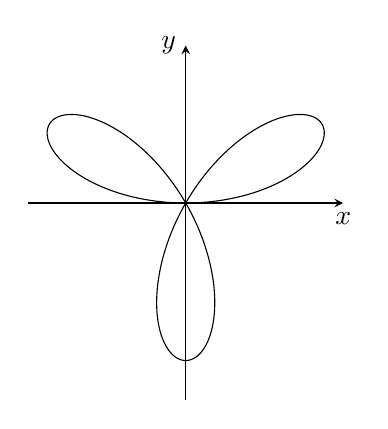
\begin{tikzpicture}[
>=stealth,
]
\draw[->] (-2,0) to (2,0)node[below]{$ x $};
\draw[->] (0,-2.5) to (0,2)node[left]{$ y $};
\draw[domain=0:360,samples=1000,scale=1] plot (\x:{2*sin(3*\x)});
\end{tikzpicture}
\caption{玫瑰线}
\end{figure}
\item 阿基米德螺线\par
$ r=a\theta (a>0,\theta \ge 0) $
\begin{figure}[H]
\centering
\begin{tikzpicture}[
>=stealth,
]
\draw[->] (0,0)node[left]{$ 0 $} to (3,0)node[below]{$ x $};
\draw[domain=0:360,samples=1000,scale=.2] plot (\x:{2*(\x/180*pi)});
\end{tikzpicture}
\caption{阿基米德螺线}
\end{figure}
\item 伯努利双纽线\par
$ r^{2}=a^{2}\cos 2\theta(a>0) $或$ r^{2}=a^{2}\sin 2\theta(a>0) $.
\begin{figure}[H]
\centering
\begin{subfigure}{.475\linewidth}
\centering
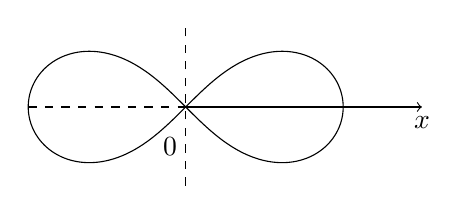
\begin{tikzpicture}
\draw[->] (0,0) to (3,0)node[below]{$ x $};
\node at (-.2,-.5){$ 0 $};
\draw[dashed] (0,-1) to (0,1);
\draw[dashed] (-2,0) to (0,0);
\draw[domain=0:45,samples=1000] plot (\x:{sqrt(4*cos(2*\x))});
\draw[domain=135:225,samples=1000] plot (\x:{sqrt(4*cos(2*\x))});
\draw[domain=315:360,samples=1000] plot (\x:{sqrt(4*cos(2*\x))});
\end{tikzpicture}
\caption{$ r^{2}=a^{2}\cos 2\theta $}
\end{subfigure}
\hfill
\begin{subfigure}{.475\linewidth}
\centering
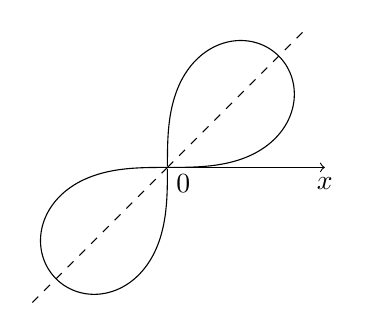
\begin{tikzpicture}
\draw[->] (0,0) to (2,0)node[below]{$ x $};
\node at (.2,-.2){$ 0 $};
\draw[domain=0:90,samples=1000,] plot (\x:{sqrt(4*sin(2*\x))});
\draw[domain=180:270,samples=1000,] plot (\x:{sqrt(4*sin(2*\x))});
\draw[dashed] (0,0) to (45:2.5);
\draw[dashed] (0,0) to (225:2.5);
\end{tikzpicture}
\caption{$ r^{2}=a^{2}\sin 2\theta $}
\end{subfigure}
\caption{伯努利双纽线}
\end{figure}
\end{enumerate}
\end{enumerate}
\subsubsection{参数方程}
\begin{enumerate}
\item 摆线\par
\begin{equation*}
\scaleleftright[6pt]{\biggl\{}{
\begin{aligned}
& x=r(t-\sin t) \\
& y=r(1-\cos t)
\end{aligned}
}{.}
\end{equation*}
\begin{figure}[H]
\centering
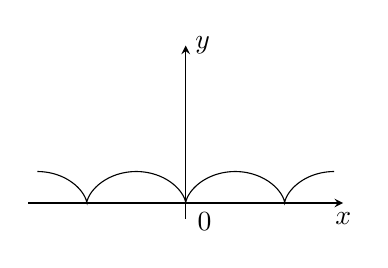
\begin{tikzpicture}[
>=stealth,
scale=2,
]
\draw[->] (-1,0) to (1,0)node[below]{$ x $};
\draw[->] (0,-.1) to (0,1)node[right]{$ y $};
\node at (.12,-.12){$ 0 $};
\draw[domain=-540:540][samples=1000] plot({(\x/180*pi-sin(\x))*0.1},{(1-cos(\x))*0.1});
\end{tikzpicture}
\caption{摆线}
\end{figure}
\item 星形线\par
\begin{equation*}
\scaleleftright[6pt]{\biggl\{}{
\begin{aligned}
& x=r\cos^{3}t \\
& y=r\sin^{3}t
\end{aligned}
}{.}
\end{equation*}
\begin{figure}[H]
\centering
\begin{tikzpicture}[
>=stealth,
scale=2,
]
\draw[->] (-1,0) to (1.2,0)node[below]{$ x $};
\draw[->] (0,-1) to (0,1.2)node[right]{$ y $};
\node at (.12,-.12){$ 0 $};
\draw[domain=0:360][samples=1000] plot({(cos(\x))^3},{(sin(\x))^3});
\end{tikzpicture}
\caption{星形线}
\end{figure}
\end{enumerate}
\subsection{常用基础知识}
\subsubsection{数列}
\begin{enumerate}
\item 等差数列\par
首项为$ a_{1} $,公差为$ d(d\neq 0) $的数列$ a_{1},a_{1}+d,a_{1}+2d,...,a_{1}+(n-1)d,... $.
\begin{enumerate}
\item 通项公式: $ a_{n}=a_{1}+(n-1)d $
\item 前$ n $项的和: $ S_{n}=\frac{n}{2}(a_{1}+a_{n})=\frac{n}{2}[2a_{1}+(n-1)d] $
\end{enumerate}
\item 等比数列\par
首项为$ a_{1} $, 公比为$ r(r\neq 0) $的数列$ a_{1},a_{1}r,...,a_{1}r^{n-1},... $.
\begin{enumerate}
\item 通项公式: $ a_{n}=a_{1}r^{n-1} $
\item 前$ n $项的和$ S_{n}=\scaleleftright[6pt]{\biggl\{}{\begin{aligned}
& na_{1}\ & r=1 \\
& \frac{a_{1}(1-r^{n})}{1-r} & r\neq 1
\end{aligned}}{.} $
\item 一些常见数列前$ n $项的和\par
\begin{enumerate}
\item $ \sum_{k=1}^{n}k=1+2+3+...+n=\frac{n(1+n)}{2} $
\item $ \sum_{k=1}^{n}k^{2}=1^{2}+2^{2}+...+n^{2}=\frac{n(n+1)(2n+1)}{6} $
\item $ \sum_{k=1}^{n}\frac{1}{k(k+1)}=\frac{1}{1\times 2}+\frac{1}{2\times 3}+...+\frac{1}{n(n+1)}=\frac{n}{n+1} $
\end{enumerate}
\end{enumerate}
\end{enumerate}
\subsubsection{三角函数}
\begin{enumerate}
\item 三角函数的基本关系
\[ \begin{split}&\csc \alpha=\frac{1}{\sin \alpha},\ \sec \alpha=\frac{1}{\cos \alpha},\ \cot \alpha=\frac{1}{\tan \alpha}\\& \sin^{2}\alpha +\cos^{2}\alpha =1,\ 1+\tan^{2}\alpha = \sec^{2}\alpha,\ 1+\cot^{2}\alpha =\csc^{2}\alpha\\ &\tan \alpha=\frac{\sin \alpha}{\cos \alpha},\ \cot \alpha=\frac{\cos \alpha}{\sin \alpha}\end{split}\]
\item 重要公式
\item 倍角公式
\[ \begin{split}
& \sin 2\alpha=2\sin \alpha \cos \alpha,\ \cos 2\alpha =\cos^{2}\alpha -\sin^{2}\alpha =1-2\sin^{2}\alpha\\&=2\cos^{2}\alpha -1,\ \tan 2\alpha =\frac{2\tan \alpha}{1-\tan^{2}\alpha}
\end{split} \]
\item 半角公式
\[ \begin{split}
& \sin^{2}\frac{\alpha}{2}=\frac{1}{2}(1-\cos \alpha),\ \cos^{2}\frac{\alpha}{2}=\frac{1}{2}(1+\cos \alpha) \\
& \tan \frac{\alpha}{2}=\frac{1-\cos \alpha}{\sin \alpha}=\frac{\sin \alpha}{1+\cos \alpha}=\pm \sqrt{\frac{1-\cos \alpha}{1+\cos \alpha}}
\end{split} \]
\item 和差公式
\[ \begin{split}
& \sin(\alpha \pm \beta)=\sin\alpha\cos\beta \pm \cos\alpha\sin\beta \\
& \cos(\alpha \pm \beta)=\cos\alpha\cos\beta \mp \sin\alpha\sin\beta \\
& \tan(\alpha \pm \beta)=\frac{\tan\alpha \pm \tan\beta}{1 \mp \tan\alpha\tan\beta}
\end{split} \]
\item 积化和差公式
\[ \begin{split}
& \sin\alpha\cos\beta = \frac{1}{2}[\sin(\alpha + \beta) + \sin(\alpha - \beta)] \\
& \cos\alpha\sin\beta = \frac{1}{2}[\sin(\alpha + \beta) - \sin(\alpha - \beta)] \\
& \cos\alpha\cos\beta = \frac{1}{2}[\cos(\alpha + \beta) + \cos(\alpha - \beta)] \\
& \sin\alpha\sin\beta = -\frac{1}{2}[\cos(\alpha + \beta) - \cos(\alpha - \beta)] \\
\end{split} \]
\item 和差化积公式
\[ \begin{split}
& \sin\alpha + \sin\beta = 2\sin\frac{\alpha+\beta}{2}\cos\frac{\alpha - \beta}{2} \\
& \sin\alpha - \sin\beta = 2\cos\frac{\alpha+\beta}{2}\sin\frac{\alpha - \beta}{2} \\
& \cos\alpha + \cos\beta = 2\cos\frac{\alpha+\beta}{2}\cos\frac{\alpha - \beta}{2} \\
& \cos\alpha - \cos\beta = -2\sin\frac{\alpha+\beta}{2}\sin\frac{\alpha - \beta}{2} \\
\end{split} \]
\item 万能公式\par
若$ u=\tan \frac{x}{2}(-\pi<x<\pi) $, 则$ \sin x=\frac{2u}{1+u^{2}} $, $ \cos x=\frac{1-u^{2}}{1+u^{2}} $.
\end{enumerate}
\subsubsection{指数运算法则}
\vspace*{-2em}
\[ \begin{split}
& a^{\alpha}\cdot a^{\beta}=a^{\alpha + \beta},\  \frac{a^{\alpha}}{a^{\beta}}=a^{\alpha-\beta} \\
& (a^{\alpha})^{\beta}=a^{\alpha \beta},\ (ab)^{\alpha}=a^{\alpha}b^{\alpha},\ (\frac{a}{b})^{\alpha}=\frac{a^{\alpha}}{b^{\alpha}}
\end{split} \]
\subsubsection{对数运算法则}
\begin{enumerate}
\item $ \log_{a}(MN)=\log_{a}M+\log_{a}N  $
\item $ \log_{a}\frac{M}{N}=\log_{a}M-\log_{a}N $
\item $ \log_{a}^{n}=n\log_{a}M $
\item $ \log_{a}\sqrt[n]{M}=\frac{1}{n}\log_{a}M $
\end{enumerate}
\subsubsection{一元二次方程基础}
\begin{enumerate}
\item 一元二次方程: $ ax^{2}+bx+c=0(a\neq 0) $
\item 根的公式: $ x_{1,2}=\frac{-b\pm \sqrt{b^{2}-4ac}}{2a} $
\item 根和系数的关系: $ x_{1}+x_{2}=-\frac{b}{a},\ x_{1}x_{2}=\frac{c}{a} $
\item 判别式: $ \Delta=b^{2}-4ac $
\item 抛物线定点坐标: $ (-\frac{b}{2a},c-\frac{b^{2}}{4a}) $
\end{enumerate}
\subsubsection{因式分解公式}
\begin{enumerate}
\item $ (a+b)^{2}=a^{2}+b^{2}+2ab $
\item $ (a-b)^{2}=a^{2}+b^{2}-2ab $
\item $ (a+b)^{3}=a^{3}+3a^{2}b+3b^{2}a+b^{3} $
\item $ (a-b)^{3}=a^{3}-3a^{2}b+3b^{2}a-b^{3} $
\item $ a^{3}+b^{3}=(a+b)(a^{2}-ab+b^{2}) $
\item $ a^{3}-b^{3}=(a-b)(a^{2}+ab+b^{2}) $
\item $ a^{2}-b^{2}=(a+b)(a-b) $
\item 二项式定理: $ (a+b)^{n}=\sum_{k=0}^{n}C_{n}^{k}a^{n-k}b^{k} $
\end{enumerate}
\subsubsection{阶乘和双阶乘}
\begin{enumerate}
\item $ n!=1\cdot 2\cdot 3\cdot ... \cdot n $, 规定$ 0!=1 $
\item $ (2n)!!=2\cdot 4\cdot 6\cdot ... \cdot (2n)=2^{n}n! $
\item $ 2(n-1)!!=1\cdot 3\cdot 5\cdot ... \cdot (2n-1) $
\end{enumerate}
\subsubsection{常用不等式}
\begin{enumerate}
\item 设$ a,b $为实数, 则有:
\begin{enumerate}
\item $ |a\pm b|\le |a|+|b| $
\item $ ||a|-|b||\le |a-b| $
\end{enumerate}
\item $ \sqrt{ab}\le \frac{a+b}{2}\le \sqrt{\frac{a^{2}+b^{2}}{2}}(a,b>0) $
\item 设$ a>b>0 $, 则$ \scaleleftright[6pt]{\biggl\{}{\begin{aligned}
& \text{当}n>0\text{时}, a^{n}>b^{n} \\
& \text{当}n<0\text{时}, a^{n}<b^{n}
\end{aligned}}{.} $
\item 若$ 0<a<x<b,0<c<y<d $, 则$ \frac{c}{b}<\frac{y}{x}<\frac{d}{a} $
\item $ \sin x<x<\tan x(0<x<\frac{\pi}{2}) $
\item $ \sin x<x(x>0) $
\item $ \arctan x\le x\le \arcsin x(0\le x\le 1)$
\item $ e^{x}\ge x+1(\forall x) $
\item $ x-1\ge \ln x(x>0) $
\item $ \frac{1}{1+x}<\ln (1+\frac{1}{x})<\frac{1}{x}(x>0) $
\end{enumerate}
\section{习题}
\subsection{复合函数}
复合函数会结合分段函数或者是其定义域考, 注意这里的定义域是$ x $的范围不是括号里面表达式的范围. 如: $ f(x+1) $的定义域为$ [0,1] $, 则$ x\in [0,1], x+1\in [1,2] $.
\subsection{函数的性态}
这里常考的是有界. 要清楚有界的三个充分条件:
\begin{enumerate}
\item 函数在$ [a,b] $内连续, 则有界
\item 函数在$ (a,b) $内连续, 且函数在$ a $点处的右极限存在, 在$ b $点处的左极限存在(特别是这个, 经常考证明极限是否存在, $ a $或者$ b $其中一个是$ \infty $也成立)
\item $ f'(x) $在$ I $上有界, 则$ f(x) $在$ I $上有界
\end{enumerate}\par
此外, (局部)保号性也是经常考的, 要清楚脱帽和戴帽规则, 说白了:
\begin{enumerate}
\item 脱帽: $ \lim\limits_{x \rightarrow x_{0}}f(x)>0\Rightarrow \exists \xi>0, \text{当}x\in \mathring{U}(x_{0}, \xi)\text{时}, \text{有}f(x)>0 $
\item 戴帽: $ \exists \xi>0, \text{当}x\in \mathring{U}(x_{0}, \xi)\text{时}, f(x)\ge 0\Rightarrow \lim\limits_{x \rightarrow x_{0}}f(x)\ge 0 $
\end{enumerate}
\chapter{数列极限}
\section{基础知识}
\subsection{数列极限的定义}
设$ \{x_{n}\} $为一数列, 若存在常数$ a $, 对于任意的$ \epsilon >0 $, 总存在正整数$ N $, 使得当$ n>N $的时候, $ |x_{n}-a|<\epsilon $恒成立, 则称数$ a $是数列$ \{x_{n}\} $的极限, 或者称数列$ \{x_{n}\} $收敛于$ a $, 记为
\begin{equation*}
\lim_{n\rightarrow \infty} x_{n} = a\ or\ x_{n}\rightarrow a(n\rightarrow \infty).
\end{equation*}\par
\begin{tcolorbox}
\begin{enumerate}
\item 至多有$ N $个项会落在$ (a-\epsilon,a+\epsilon) $之外
\item 数列极限的存在性和大小和前$ N $项无关
\item 子数列和父数列的极限相同, 即$ \lim\limits_{n \rightarrow \infty}x_{n}=\lim\limits_{k \rightarrow \infty}x_{2k-1}=\lim\limits_{k \rightarrow \infty}x_{2k+1}=a $
\item 若$ \lim\limits_{n \rightarrow \infty}a_{n}=a\Rightarrow \lim\limits_{n \rightarrow \infty}|a_{n}|=|a| $
\item $ \lim\limits_{n \rightarrow \infty}\sqrt[n]{a_{1}^{n}+a_{2}^{n}+...+a_{m}^{n}}=\mathrm{max}_{1\le i\le m}\{a_{i}\}, \text{其中}\ a_{i}>0 $
\end{enumerate}
\end{tcolorbox}
\subsection{收敛数列的性质}
\begin{enumerate}
\item 唯一性: 若数列存在极限, 则极限唯一
\item 有界性: 若数列存在极限, 则数列有界
\item 保号性
\begin{enumerate}
\item 脱帽: 设有数列$ \{x_{n}\} $, 若$ \lim\limits_{n\rightarrow \infty}x_{n}=a>0(\text{或}<0)\Rightarrow $ 存在正整数$ N $, 当$ n>N $时, 有$ x_{n}>0(\text{或}x_{n}<0) $
\item 戴帽: 设有数列$ \{x_{n}\} $, 若存在正整数$ N $, 当$ n>N $时, 有$ x_{n}\ge 0 $, 且数列存在极限$ \Rightarrow \lim\limits_{n\rightarrow \infty}x_{n}=a\ge 0 $
\end{enumerate}
\end{enumerate}
\subsection{极限运算规则}
设$ \lim\limits_{n\rightarrow \infty}x_{n}=a, \lim\limits_{n\rightarrow \infty}y_{n}=b $, 则
\begin{enumerate}
\item $ \lim\limits_{n\rightarrow \infty}(x_{n}\pm y_{n})=a\pm b $
\item $ \lim\limits_{n\rightarrow \infty}x_{n}y_{n}=ab $
\item 若$ b\neq 0, y_{n}\neq 0 \Rightarrow \lim\limits_{n\rightarrow \infty}\frac{x_{n}}{y_{n}}=\frac{a}{b}$
\end{enumerate}\par
注意, 当$ \lim\limits f(x), \lim\limits g(x) $其中一个存在, 另一个不存在的时候, 上述左边的极限一定不存在. 当$ \lim\limits f(x), \lim\limits g(x) $两个都不存在的时候, 左边的极限不一定不存在.
\subsection{夹逼准则}
若数列$ \{x_{n}\}, \{y_{n}\} $及$ \{z_{n}\} $满足条件:
\begin{enumerate}
\item $ y_{n}\le x_{n}\le z_{n}(n=1,2,3...) $
\item $ \lim\limits_{n\rightarrow \infty}y_{n}=a, \lim\limits_{n\rightarrow \infty}z_{n}=a $
\end{enumerate}\par
则数列$ \{x_{n}\} $的极限存在, 且$ \lim\limits_{n\rightarrow \infty}x_{n}=a $.
\subsection{单调有界准则}
单调有界数列必有极限.
\section{习题}
\subsection{求解数列极限}
\subsubsection{不定式}
与求函数不定式极限的方法完全相同, 但是对数列极限不能直接用洛必达法则, 必须先转化为函数, 再用洛必达法则.
\subsection{$ n $项和的数列极限}
常用二种方法:
\begin{enumerate}
\item 夹逼定理: 变化部分是主体同量级, 用夹逼原理
\item 转化为$ 0-1 $上的定积分: 变化部分是主体次量级, 用定积分定义
\end{enumerate}
\subsection{$ n $项连乘的数列极限}
常用两种方法:
\begin{enumerate}
\item 夹逼原理
\item 取对数化为$ n $项和
\end{enumerate}
\subsection{递推关系定义的数列}
用单调有界准则做, 具体见\hyperref[单调有界准则算极限]{单调有界准则算极限}.
\chapter{函数极限}
\section{基础知识}
\subsection{邻域}
\subsubsection{一维}
\begin{enumerate}
\item 邻域: 点$ x_{0} $的邻域为数轴上以$ x_{0} $为中心的任何开区间, 记作$ U(x_{0}) $
\item $ \delta $邻域: 点$ x_{0} $的$ \delta $邻域为$ (x_{0}-\delta,x_{0}+\delta) $, 记作$ U(x_{0},\delta) $
\item 去心$ \delta $邻域: 点$ x_{0} $的去心$ \delta $邻域为$ (x_{0}-\delta,x_{0})\cup (x_{0},x_{0}+\delta) $, 记作$ \mathring{U}(x_{0},\delta) $
\item 左右$ \delta $邻域
\begin{enumerate}
\item 左邻域: 点$ x_{0} $的左邻域为$ (x_{0}-\delta,x_{0}) $, 记作$ U^{+}(x_{0},\delta) $
\item 右邻域: 点$ x_{0} $的右邻域为$ (x_{0},x_{0}+\delta) $, 记作$ U^{-}(x_{0},\delta) $
\end{enumerate}
\end{enumerate}
\subsubsection{二维}
\begin{enumerate}
\item $ \delta $邻域: 与点$ P_{0}(x_{0},y_{0}) $的距离小于$ \delta $的点$ P(x,y) $的全体, 称为点$ P_{0} $的$ \delta $邻域, 记作$ U(P_{0},\delta) $
\item 去心$ \delta $邻域: 与点$ P_{0}(x_{0},y_{0}) $的距离小于$ \delta $但不等于0的点$ P(x,y) $的全体, 称为点$ P_{0} $的去心$ \delta $邻域, 记作$ \mathring{U}(P_{0},\delta) $
\end{enumerate}
\subsection{函数极限的定义}
设函数$ f(x) $在某点$ x_{0} $的某一去心邻域内有定义.
\begin{enumerate}
\item 自变量趋近于无穷大
\subitem $ \lim\limits_{x\rightarrow \infty}f(x)=A\Leftrightarrow \forall \epsilon >0, \exists X>0 $, 当$ |x|>X $时, 有$ |f(x)-A|<\epsilon $
\subitem $ \lim\limits_{x\rightarrow +\infty}f(x)=A\Leftrightarrow \forall \epsilon >0, \exists X>0 $, 当$ x>X $时, 有$ |f(x)-A|<\epsilon $
\subitem $ \lim\limits_{x\rightarrow -\infty}f(x)=A\Leftrightarrow \forall \epsilon >0, \exists X>0 $, 当$ x<-X $时, 有$ |f(x)-A|<\epsilon $
\item 自变量趋近于有限值
\subitem $ \lim\limits_{x\rightarrow x_{0}}f(x)=A\Leftrightarrow \forall \epsilon >0, \exists \xi>0 $, 当$ 0<|x-x_{0}|<\xi $时, 有$ |f(x)-A|<\epsilon $
\end{enumerate}
\subsubsection{单侧极限}
\begin{enumerate}
\item 左极限: $ \lim\limits_{x\rightarrow x_{0}^{-}}f(x)=A\ or\ f(x_{0}^{-})=A $
\item 右极限: $ \lim\limits_{x\rightarrow x_{0}^{+}}f(x)=A\ or\ f(x_{0}^{+})=A $
\end{enumerate}
\begin{tcolorbox}
要分左右求极限的问题主要有三种:
\begin{enumerate}
\item 分段函数在分界点的极限
\item $ e^{\infty} $的极限
\item $ \arctan \infty $的极限
\end{enumerate}
\end{tcolorbox}
\subsubsection{充要条件}
函数$ f(x) $在点$ x_{0} $处有极限的充要条件分别有:
\begin{enumerate}
\item $ \lim\limits_{x\rightarrow x_{0}}f(x)=A\Leftrightarrow \lim\limits_{x\rightarrow x_{0}^{-}}f(x)=\lim\limits_{x\rightarrow x_{0}^{+}}f(x)=A $
\item $ \lim\limits_{x\rightarrow x_{0}}f(x)=A\Leftrightarrow f(x)=A+\alpha(x), \lim\limits_{x\rightarrow x_{0}}\alpha(x)=0 $
\end{enumerate}
\subsubsection{极限不存在}
极限不存在$ \Leftrightarrow \lim\limits f(x)=\infty $.
\subsubsection{函数收敛}
函数收敛$ \Leftrightarrow \lim\limits_{x \rightarrow x_{0}}f(x)=C $($ C $为常数).
\subsection{收敛函数的性质}
\begin{enumerate}
\item 唯一性: 若函数存在极限, 则极限唯一
\item 局部有界性: 若函数存在极限, 则函数在某一区间内有界
\item 局部保号性
\begin{enumerate}
\item 脱帽: 设有函数$ f(x) $, 若$ \lim\limits_{x\rightarrow x_{0}}f(x)=A>0(\text{或}A<0) \Rightarrow $ 存在常数$ \delta $, 当$ 0<|x-x_{0}|<\delta $时, 有$ f(x)>0(\text{或}f(x)<0) $
\item 戴帽: 设有函数$ f(x) $, 若存在常数$ \delta $, 当$ 0<|x-x_{0}|<\delta $时, 有$ f(x)\ge 0(\text{或}f(x)\le 0) \Rightarrow \lim\limits_{x\rightarrow x_{0}}f(x)=A\ge 0(\text{或}\le 0) $
\end{enumerate}
\end{enumerate}
\begin{tcolorbox}
由局部保号性可以得到局部保序性: 设$ \lim\limits_{x \rightarrow x_{0}}f(x)=A, \lim\limits_{x \rightarrow x_{0}}g(x)=B $
\begin{enumerate}
\item 脱帽: 若$ A>B\Rightarrow \exists \delta>0 $, 当$ 0<|x-x_{0}|<\delta $时, 有$ f(x)>g(x) $.
\item 戴帽: 若$ \exists \delta>0 $, 当$ 0<|x-x_{0}|<\delta $时, 有$ f(x)\ge g(x)\Rightarrow A\ge B $
\end{enumerate}
\end{tcolorbox}
\subsection{极限运算法则}
设$ \lim\limits_{x\rightarrow x_{0}}f(x)=A, \lim\limits_{x\rightarrow x_{0}}g(x)=B $, 则
\begin{enumerate}
\item $ \lim\limits_{x\rightarrow x_{0}}[kf(x)\pm lg(x)]=k \lim\limits_{x\rightarrow x_{0}}f(x)\pm l \lim\limits_{x\rightarrow x_{0}}g(x)=kA\pm lB $, 其中$ k,l $为常数
\item $ \lim\limits_{x\rightarrow x_{0}}[f(x)\cdot g(x)]=\lim\limits_{x\rightarrow x_{0}}f(x)\cdot \lim\limits_{x\rightarrow x_{0}}g(x)=A\cdot B $
\item $ \lim\limits_{x\rightarrow x_{0}}\frac{f(x)}{g(x)}=\frac{\lim\limits_{x\rightarrow x_{0}}f(x)}{\lim\limits_{x\rightarrow x_{0}}g(x)}=\frac{A}{B}(B\neq 0) $
\item $ \lim\limits_{x\rightarrow x_{0}}[f(x)]^{n}=[\lim\limits_{x\rightarrow x_{0}}f(x)]^{n} $, $ n $为正整数
\end{enumerate}\par
注意, 当$ \lim\limits f(x), \lim\limits g(x) $其中一个存在, 另一个不存在的时候, 上述左边的极限一定不存在. 当$ \lim\limits f(x), \lim\limits g(x) $两个都不存在的时候, 左边的极限不一定不存在.
\subsection{夹逼准则}\label{夹逼定理}
若函数$ f(x), g(x) $及$ h(x) $满足条件:
\begin{enumerate}
\item $ g(x)\le f(x)\le h(x) $
\item $ \lim\limits_{x\rightarrow x_{0}}g(x)=A, \lim\limits_{x\rightarrow x_{0}}h(x)=A $
\end{enumerate}\par
则函数$ f(x) $极限存在, 且$ \lim\limits_{x\rightarrow x_{0}}f(x)=A $.
\subsection{单调有界准则}
单调有界函数必有极限.
\subsection{洛必达法则}\label{洛必达法则}
\begin{enumerate}
\item $ \frac{0}{0} $: $ \lim\limits_{x\rightarrow a}\frac{f(x)}{F(x)}=\lim\limits_{x\rightarrow a}\frac{f'(x)}{F'(x)} $(或$ \lim\limits_{x\rightarrow \infty}\frac{f(x)}{F(x)}=\lim\limits_{x\rightarrow \infty}\frac{f'(x)}{F'(x)} $), 需要以下条件:
\begin{enumerate}
\item 若$ x\rightarrow a(\text{或}x\rightarrow \infty) $时, 函数$ f(x) $及$ F(x) $都趋近于$ 0 $
\item 且$ f'(x) $及$ F'(x) $在点$ a $的去心邻域内(或当$ |x|>X $时, $ X $为充分大的正数)存在, 且$ F'(x)\neq 0 $
\item $ \lim\limits_{x\rightarrow a}\frac{f'(x)}{F'(x)} $(或$ \lim\limits_{x\rightarrow \infty}\frac{f'(x)}{F'(x)} $)存在或者无穷大
\end{enumerate}
\item $ \frac{\infty}{\infty} $: $ \lim\limits_{x\rightarrow a}\frac{f(x)}{F(x)}=\lim\limits_{x\rightarrow a}\frac{f'(x)}{F'(x)} $(或$ \lim\limits_{x\rightarrow \infty}\frac{f(x)}{F(x)}=\lim\limits_{x\rightarrow \infty}\frac{f'(x)}{F'(x)} $), 需要以下条件:
\begin{enumerate}
\item 若$ x\rightarrow a(\text{或}x\rightarrow \infty) $时, 函数$ f(x) $及$ F(x) $都趋近于$ \infty $
\item 且$ f'(x) $及$ F'(x) $在点$ a $的去心邻域内(或当$ |x|>X $时, $ X $为充分大的正数)存在, 且$ F'(x)\neq 0 $
\item $ \lim\limits_{x\rightarrow a}\frac{f'(x)}{F'(x)} $(或$ \lim\limits_{x\rightarrow \infty}\frac{f'(x)}{F'(x)} $)存在或者无穷大
\end{enumerate}
\end{enumerate}
\begin{tcolorbox}
对于$ \lim\limits_{x\rightarrow a}\frac{f(x)}{F(x)}=\lim\limits_{x\rightarrow a}\frac{f'(x)}{F'(x)} $, 右存在, 则左存在; 但左存在, 并不意味着右存在
\end{tcolorbox}
\subsection{泰勒公式}
\subsubsection{泰勒公式表}
\begin{multicols}{2}
\begin{itemize}
\item $ \sin x=x-\frac{x^{3}}{3!}+o(x^{3}) $
\item $ e^{x}=1+x+\frac{x^{2}}{2!}+\frac{x^{3}}{3!}+o(x^{3}) $
\item $ \arcsin x=x+\frac{x^{3}}{3!}+o(x^{3}) $
\item $ \tan x=x+\frac{x^{3}}{3}+o(x^{3}) $
\item $ \cos x=1-\frac{x^{2}}{2!}+\frac{x^{4}}{4!}+o(x^{4}) $
\item $ ln(1+x)=x-\frac{x^{2}}{2}+\frac{x^{3}}{3}+o(x^{3}) $
\item $ \arctan x=x-\frac{x^{3}}{3}+o(x^{3}) $
\item $ (1+x)^{\alpha}=1+\alpha x+\frac{\alpha (\alpha -1)}{2!}x^{2}+\frac{\alpha (\alpha -1)(\alpha -2)}{3!}x^{3}+o(x^{3}) $
\end{itemize}
\end{multicols}
\subsubsection{用泰勒公式求极限}
\begin{enumerate}
\item $ \frac{A}{B} $: 适用于``上下同阶''的原则 \par
如果分母(或者分子)是$ x $的$ k $此幂, 则应该把分子(或分母)展开到$ x $的$ k $次幂.
\item $ A-B $: 适用于幂次最低原则 \par
将$ A, B $分别展开到它们的系数不相等的$ x $的最低次幂为止.
\end{enumerate}
\subsection{无穷小}
\subsubsection{无穷小定义}
如果当$ x\rightarrow x_{0}(\text{或}x\rightarrow \infty) $函数$ f(x) $的极限为零$ \Rightarrow  $函数$ f(x) $为当$ x \rightarrow x_{0}(\text{或}x \rightarrow \infty ) $时的无穷小.
\subsubsection{无穷小的比阶}\label{无穷小的比阶}
\begin{enumerate}
\item 高阶无穷小: $ \lim\limits \frac{\alpha(x)}{\beta(x)}=0 $, $ \alpha(x) $是$ \beta(x) $的高阶无穷小, 记作$ \alpha(x)=o(\beta(x)) $
\item 低阶无穷小: $ \lim\limits \frac{\alpha(x)}{\beta(x)}=\infty $, $ \alpha(x) $是$ \beta(x) $的低阶无穷小
\item 同阶无穷小: $ \lim\limits \frac{\alpha(x)}{\beta(x)}=c(\neq 0) $, $ \alpha(x) $是$ \beta(x) $的同阶无穷小
\item 等价无穷小: $ \lim\limits \frac{\alpha(x)}{\beta(x)}=1 $, $ \alpha(x) $是$ \beta(x) $的等阶无穷小
\item $ k $阶无穷小: $ \lim\limits \frac{\alpha(x)}{[\beta(x)]^{k}}=c\neq 0, k>0 $, $ \alpha(x) $是$ \beta(x) $的$ k $阶无穷小
\end{enumerate}\par
通常我们所说的$ n $阶无穷小的含义是$ \lim\limits \frac{\alpha(x)}{x^{n}}=c\neq 0 $, 则$ \alpha(x) $就是$ n $阶无穷小.
\begin{tcolorbox}
并不是任意两个无穷小都可以进行比阶的, 如: 当$ x \rightarrow 0 $的时候, $ \lim\limits_{x\rightarrow 0}\frac{x\sin \frac{1}{x}}{x^{2}}=\lim\limits_{x\rightarrow 0}\frac{1}{x}\sin \frac{1}{x} $不存在 \par \vspace{.5em}
\textbf{常用结论: } 若$ f(x) $在$ x=0 $的某领域内连续, 且当$ x\rightarrow 0 $时$ f(x) $是$ x $的$ m $阶无穷小, $ \varphi(x) $是$ x $的$ n $阶无穷小, 则当$ x\rightarrow 0 $时, $ F(x)=\displaystyle\int_{0}^{\varphi(x)}\hspace{.2em}f(t)\mathrm{d}t $是$ x $的$ n(m+1) $阶无穷小.(2020和2021两年第一题都可以用这个秒杀), 如$ \displaystyle\int_{\sin x}^{1-\sqrt{\cos x}}\hspace{.2em}\ln (1+t^{3})\mathrm{d}t=\displaystyle\int_{0}^{1-\sqrt{\cos x}}\hspace{.2em}\ln(1+t^{3})\mathrm{d}t-\displaystyle\int_{0}^{\sin x}\hspace{.2em}\ln(1+t^{3})\mathrm{d}t $, $ \displaystyle\int_{0}^{1-\sqrt{\cos x}}\hspace{.2em}\ln(1+t^{3})\mathrm{d}t $是$ 2\times (3+1)=8 $阶, $ \displaystyle\int_{0}^{\sin x}\hspace{.2em}\ln(1+t^{3})\mathrm{d}t $是$ 1\times(3+1)=4 $阶, 由于$ x\rightarrow 0 $, 故后者是老大, 所以$ \displaystyle\int_{\sin x}^{1-\sqrt{\cos x}}\hspace{.2em}\ln (1+t^{3})\mathrm{d}t $是$ 4 $阶.
\end{tcolorbox}
\subsubsection{无穷小的运算规则}
\begin{enumerate}
\item 有限个无穷小的和(差)是无穷小
\item 有限个无穷小的乘积还是无穷小
\item 有界函数和无穷小的乘积还是无穷小
\item 无穷小的运算 \par 
\begin{enumerate}
\item $ o(x^{m})\pm o(x^{n})=o(x^{min\{m,n}\}) $
\item $ o(x^{m})\cdot o(x^{n})=o(x^{m+n}), x^{m}\cdot o(x^{n})=o(x^{m+n}) $
\item $ o(x^{m})=o(kx^{m})=k\cdot o(x^{m}) $
\end{enumerate}
\end{enumerate}
\subsubsection{等价无穷小表}
\begin{multicols}{2}
\begin{itemize}
\item $ \sin x\sim x $
\item $ \arcsin x\sim x $
\item $ \ln (1+x)\sim x $
\item $ \alpha^{x}-1\sim x\ln a $
\item $ \tan x\sim x $
\item $ \arctan x\sim x $
\item $ e^{x}-1\sim x $
\item $ (1+x)^{\alpha}-1\sim \alpha x $
\item $ 1-\cos x\sim \frac{1}{2}x^{2} $
\item $ 1-\cos^{\alpha} x\sim \frac{\alpha}{2}x^{2} $
\end{itemize}
\end{multicols}
\begin{tcolorbox}
$ (1+x)^{\alpha}-1\sim \alpha x $这个式子可以推广为$ (1+\alpha(x))^{\beta(x)}-1\sim \alpha (x)\beta (x) $, 条件是$ \alpha(x)\rightarrow 0, \alpha(x)\beta(x)\rightarrow 0 $
\end{tcolorbox}
\subsubsection{变上限积分的无穷小替换}
设$ f(x) $和$ g(x) $在$ x=0 $的某邻域内连续, 且$ \lim\limits_{x \rightarrow 0}\frac{f(x)}{g(x)}=1, \lim\limits_{x \rightarrow 0}\varphi(x)=0 $, 则:
\begin{equation*}
\displaystyle\int_{0}^{\varphi(x)}\hspace{.2em}f(t)\mathrm{d}t\sim \displaystyle\int_{0}^{\varphi(x)}\hspace{.2em}g(t)\mathrm{d}t
\end{equation*}\par
注意, 这里的$ f(x) $和$ g(x) $没说都趋向于$ 0 $, 可以都趋向于同一个常数, 结果$ \lim\limits_{x \rightarrow 0}\frac{f(x)}{g(x)} $也是$ 1 $.
\subsection{无穷大}
\subsubsection{无穷大的概念}
若$ \lim\limits_{x \rightarrow x_{0}}f(x)=\infty $或$ \lim\limits_{x \rightarrow \infty}f(x)=\infty $, 则称$ f(x) $为$ x\rightarrow x_{0} $或$ x\rightarrow \infty $时的无穷大.
\subsubsection{常用的一些无穷大的比较}
\begin{enumerate}
\item 当$ x\rightarrow +\infty $时, $ \ln^{\alpha}x<<x^{\beta}<<a^{x}\ (\alpha>0, \beta>0, a>1) $
\item 当$ n\rightarrow \infty $时, $ \ln^{\alpha}n<<n^{\beta}<<a^{n}<<n!<<n^{n}\ (\alpha>0, \beta>0, a>1) $
\end{enumerate}
\subsubsection{无穷大量和无界变量的关系}
无穷大$ \Rightarrow $无界变量.\par
无穷大量: $ \forall M>0, \exists X, $当$ x>X $时, 恒有$ |f(x)|>M $ \par
无界量: $ \forall M>0, \exists X, $, 使$ |f(X)|>M $
\begin{tcolorbox}
\textbf{无界$ \times $无界不一定是无界}:\par 令$ x_{n}=0,2,0,4,...\ y_{n}=1,0,3,0,...\ $, 但是$ \lim\limits_{x \rightarrow \infty}x_{n}\times y_{n}=0 $, 这里就用到了无界量和无穷大量的区别.\par \vspace{.5em}
\textbf{有界量$ \times $无穷小一定是无穷小}: 根据无穷小的性质.\par \vspace{.5em}
无穷大的定义中, 是在$ n>N $的时候, 恒有$ |x_{N}|>M $, 注意是带有绝对值的, 例如, 对于$ x_{n}=(-2)^{n} $来说, 虽然它是震荡的, 但它仍是无穷大, 而$ x_{n}=(-1)^{n} $就不是无穷大.
\end{tcolorbox}
\subsubsection{无穷大和无穷小的关系}
\section{习题}
\subsection{极限的概念/性质/存在准则}
首先记住一条结论: $ \lim\limits_{n \rightarrow \infty}a_{n}=a\Rightarrow \lim\limits_{n \rightarrow \infty}|a_{n}|=|a| $.\par
这里常考的是直接举反例, 或者是结合极限运算的前提考察.
\subsection{求解极限}
首先, 要明确一点的是, 如果极限中的某一部分可以直接求出来的话, 是可以用结果替代掉的.
\subsubsection{极限的基本运算}
这里用到的是极限的四个运算法则:
\begin{enumerate}
\item $ \lim\limits (f(x)\pm g(x))=\lim\limits f(x)\pm \lim\limits g(x) $
\item $ \lim\limits (f(x)\cdot g(x))=\lim\limits f(x)\cdot \lim\limits g(x) $
\item $ \lim\limits \frac{f(x)}{g(x)}=\frac{\lim\limits f(x)}{\lim\limits g(x)} $, $ g(x)\neq 0, \lim\limits g(x)\neq 0 $
\item $ (\lim\limits f(x))^{n}={\lim\limits}^{n}f(x) $
\end{enumerate}\par
\begin{tcolorbox}
要特别注意的是:\par
$ \lim\limits f(x), \lim\limits g(x) $中两个都不存在 $ \Rightarrow\lim\limits f(x)\pm \lim\limits g(x) $可能存在.\par
$ \lim\limits f(x), \lim\limits g(x) $中一个存在, 另一个不存在 $ \Rightarrow \lim\limits f(x)\pm g(x) $一定不存在.
\end{tcolorbox}
\subsubsection{基本极限}
要牢记以下的基本极限:
\begin{multicols}{2}
\begin{itemize}
\item $ \lim\limits_{x \rightarrow 0}(1+x)^{\frac{1}{x}}=e $
\item $ \lim\limits_{x \rightarrow \infty}\sqrt[x]{x}=1 $
\item $ \lim\limits_{x \rightarrow 0}\frac{\sin x}{x}=1 $
\item $ \lim\limits_{x \rightarrow 0}\frac{\alpha^{x}-1}{x}=\ln \alpha $($ \alpha>1 $)
\item $ \lim\limits_{x \rightarrow 0}\frac{a_{m}x^{m}+a_{m-1}x^{m-1}+...+a_{0}}{b_{n}x^{n}+b_{n-1}x^{n-1}+...+b_{0}}=
\scaleleftright[6pt]{\biggl\{}{
\begin{aligned}
& \frac{a_{m}}{b_{n}},\ m=n \\
& 0,\ m>n \\
& \infty,\ m<n
\end{aligned}
}{.} $
\item $ \lim\limits_{n \rightarrow \infty}x^{n}=
\scaleleftright[6pt]{\biggl\{}{
\begin{aligned}
& 0,\ |x|<1 \\
& \infty,\ |x|>1 \\
& 1,\ x=1 \\
& \text{不存在},\ x=-1
\end{aligned}
}{.} $
\item $ \lim\limits_{n \rightarrow \infty}e^{nx}=
\scaleleftright[6pt]{\biggl\{}{
\begin{aligned}
& 0,\ x<0 \\
& +\infty,\ x>0 \\
& 1,\ x=0
\end{aligned}
}{.} $
\end{itemize}
\end{multicols}
\begin{tcolorbox}
\textbf{谁是老大?}\par \vspace{1em}
$ \lim\limits_{x \rightarrow 0}\frac{a_{m}x^{m}+a_{m-1}x^{m-1}+...+a_{0}}{b_{n}x^{n}+b_{n-1}x^{n-1}+...+b_{0}} $这个式子中的老大是最低阶的项, 其他的项可以忽略不看.\par \vspace{.5em} $ \lim\limits_{x \rightarrow \infty}\frac{a_{m}x^{m}+a_{m-1}x^{m-1}+...+a_{0}}{b_{n}x^{n}+b_{n-1}x^{n-1}+...+b_{0}} $这个式子中的老大是最高阶的项, 其他的项可以忽略不看.
\end{tcolorbox}
\subsubsection{等价无穷小}
{\kaishu 常用的等价无穷小}\vspace{-1em}
\begin{multicols}{2}
\begin{itemize}
\item $ \sin x\sim x $
\item $ \tan x\sim x $
\item $ \arcsin x\sim x $
\item $ \arctan x\sim x $
\item $ \ln(1+x)\sim x $
\item $ e^{x}-1\sim x $
\item $ (1+x)^{\alpha}-1\sim \alpha x $
\item $ \alpha^{x}-1\sim x\ln \alpha $
\end{itemize}
\end{multicols}
{\kaishu 等价无穷小替换的原则}\par \vspace{.5em}
设$ f(x)\sim \alpha, g(x)\sim \beta $
\begin{enumerate}
\item 乘除关系可以直接替换
\item 加减关系需要满足:
\subitem $ \lim\limits \frac{\alpha}{\beta}=A\neq 1\Rightarrow f(x)-g(x)\sim \alpha-\beta $
\subitem $ \lim\limits \frac{\alpha}{\beta}=A\neq -1\Rightarrow f(x)+g(x)\sim \alpha+\beta $
\end{enumerate}\par
\textbf{加减关系的条件换一句话说就是: 替换后加减的结果不能为$ 0 $}.
\subsubsection{泰勒公式}
{\kaishu 常用的泰勒公式}\vspace{-1em}
\begin{multicols}{2}
\begin{itemize}
\item $ \sin x=x-\frac{x^{3}}{3!}+o(x^{3}) $
\item $ \tan x=x+\frac{x^{3}}{3}+o(x^{3}) $
\item $ \cos x=1-\frac{x^{2}}{2!}+o(x^{2}) $
\item $ \arcsin x=x+\frac{x^{3}}{3!}+o(x^{3}) $
\item $ \arctan x=x-\frac{x^{3}}{3}+o(x^{3}) $
\item $ e^{x}-1=x+\frac{x^{2}}{2!}+\frac{x^{3}}{3!}+o(x^{3}) $
\item $ \ln(1+x)=x-\frac{x^{2}}{2}+\frac{x^{3}}{3}+o(x^{3}) $
\item $ (1+x)^{\alpha}-1=\alpha x+\frac{\alpha(\alpha-1)}{2!}x^{2}+\frac{\alpha(\alpha-1)(\alpha-2)}{3!}x^{3}+o(x^{3}) $
\end{itemize}
\end{multicols}\par
要注意到, 泰勒公式其实和无穷小有很大的相通性.
\subsubsection{洛必达法则}
\hyperref[洛必达法则]{洛必达法则}在前面已经介绍过, 不再赘述. 七种不定式几乎都可以用洛必达做.
\subsubsection{单调有界准则}\label{单调有界准则算极限}
单调有界准则常常用于求数列的极限, 步骤是:
\begin{enumerate}
\item 证明数列有界
\item 证明数列单调
\item 当$ n\rightarrow \infty $时, $ x_{n}=x_{n+1}=x_{n-1} $, 将关系式中的$ x_{n}, x_{n-1}, x_{n+1} $全部换成$ a $, 求解$ a $就是极限
\end{enumerate}\par
注意先后顺序, 先证明有界, 再证明单调.
\subsubsection{夹逼定理}
\hyperref[夹逼定理]{夹逼定理}在前面已经介绍过, 不再赘述. 常常会用到放缩法.
\subsubsection{定积分的含义}
\begin{equation*}
\int_{0}^{1}f(x)\mathrm{d}x=\lim\limits_{n \rightarrow \infty}\frac{1}{n}\sum_{k=1}^{n}f(\frac{k}{n})
\end{equation*}\par
其核心是提取公因子$ \frac{1}{n} $, 然后将其余部分化为$ \sum_{k=1}^{n}f(\frac{k}{n}) $.
\begin{tcolorbox}
\textbf{什么时候用定积分, 什么时候用夹逼定理}
\begin{enumerate}
\item 分母中非变化量和变化量同量级$ \Rightarrow $定积分定义
\item 分母中非变化量和变化量非同量级$ \Rightarrow $夹逼定理
\end{enumerate}
\end{tcolorbox}
\subsection{求解函数极限(七种不定式的计算)}
七种不定式中, 最基础的是$ \frac{0}{0}, \frac{\infty}{\infty} $. 其次是$ \infty-\infty, 0\cdot\infty $, 其中后者可以细分为$ 0^{0}, 1^{\infty}, \infty^{0} $.
\subsubsection{$ \frac{0}{0} $型}
三种方法:
\begin{enumerate}
\item 等价无穷小替换: 要注意加减时候等价无穷小替换的规则(结果不能为$ 0 $)
\item 泰勒公式替换: 无穷小的阶数一定要和分母的阶数保持一致
\item 洛必达法则
\end{enumerate}
\subsubsection{$ \frac{\infty}{\infty} $型}
两种方法:
\begin{enumerate}
\item 洛必达法则
\item 分母分子同处以最高阶的无穷大
\end{enumerate}
\subsubsection{$ \infty-\infty $型}
三种方法:
\begin{enumerate}
\item 分式差: 将其化为$ \frac{\infty}{\infty} $, 这里的分式指的是两个减数都要是分式, 如果没法直接化为分式, 可以进行变量代换, 强行化为分式
\item 根式差: 将根式有理化
\item 提取无穷因子: 将无穷因子作为一个整体做变量代换
\end{enumerate}
\subsubsection{$ 0\cdot \infty $型}
直接化为$ \frac{0}{0} $型或者$ \frac{\infty}{\infty} $型. 注意如果转换为$ \frac{0}{0} $之后不好求导, 可以先将$ 0\times \infty $中的$ 0 $用等价无穷小替换掉.
\subsubsection{$ 1^{\infty} $型}
如果想慢慢算, 可以用$ exp $做, 如果不想算, 直接用公式:
\begin{equation*}
\text{若}\lim\limits \alpha(x)=0, \lim\limits \beta(x)=\infty, \lim\limits \alpha(x)\beta(x)=A \text{则}\lim\limits (1+\alpha(x))^{\beta(x)}=e^{A}
\end{equation*}
\subsubsection{$ \infty^{0}, 0^{0} $型}
可以转为为$ exp $形式.
\subsubsection{$ 0-0/? $型(热门题型)}
\begin{enumerate}
\item 泰勒公式展开至与分母同阶, 或者是同次幂项相减等于$ 0 $
\item 分子中含有两个$ e $可以直接提取公因子, 若只含有一个$ e $, 可以将两一个化为$ e $的形式, 然后提取公因子
\item 分子中含有$ ln $, 可以运用对数的求导法则
\item 如果出现同一个函数的两个不同的点的函数值相减, 联想到拉格朗日中值定理
\end{enumerate}
\subsection{根据极限求参数}
已知函数(数列)极限求参数, 也是极限的计算. 可以利用等价无穷小的代换和性质, 求极限的方法结合已知条件进行求解. 常用的结论:
\begin{equation*}
\begin{aligned}
& \lim\limits \frac{\alpha(x)}{\beta(x)}=A, 若 \lim\limits \beta(x)=0\Rightarrow \lim\limits \alpha(x)=0 \\
& \lim\limits \frac{\alpha(x)}{\beta(x)}=A\neq 0, 若 \lim\limits \alpha(x)=0\Rightarrow \lim\limits \beta(x)=0
\end{aligned}
\end{equation*}
\subsection{根据极限求导数}
\subsection{无穷小的比阶确定参数}
见\hyperref[无穷小的比阶]{无穷小的比阶}, 重点注意的是$ k $阶无穷小的定义.
\chapter{函数的连续和间断}
\section{基础知识}
\subsection{连续的定义}
设函数$ f(x) $在点$ x_{0} $的某一邻域内有定义, 且有$ \lim\limits_{x\rightarrow x_{0}}f(x)=f(x_{0}) $, 则称函数$ f(x) $在点$ x_{0} $处连续.
\subsubsection{左连续和右连续}
\begin{enumerate}
\item 左连续: $ \lim\limits_{x \rightarrow x_{0}^{-}}f(x)=f(x_{0}) $
\item 右连续: $ \lim\limits_{x \rightarrow x_{0}^{+}}f(x)=f(x_{0}) $
\end{enumerate}
\subsubsection{充要条件}
极限存在(左极限=右极限)且等于函数在这个点的函数值:
\begin{equation*}
\lim\limits_{x \rightarrow x_{0}^{-}}f(x)=\lim\limits_{x \rightarrow x_{0}^{+}}f(x)=f(x_{0})
\end{equation*}
\subsection{间断点的定义}
\begin{enumerate}
\item 第一类间断点: 左极限和右极限都存在
\begin{enumerate}
\item 可去间断点(左极限$ = $右极限$ \neq $函数值): $ \lim\limits_{x\rightarrow x_{0}}f(x)=A\neq f(x_{0}) $
\item 跳跃间断点(左极限$ \neq $右极限): $ \lim\limits_{x\rightarrow x_{0}^{-}}f(x) \neq \lim\limits_{x\rightarrow x_{0}^{+}}f(x) $
\end{enumerate}
\item 第二类间断点: 左极限和右极限至少有一个不存在
\begin{enumerate}
\item 无穷间断点: $ \lim\limits_{x\rightarrow x_{0}}f(x)=\infty $
\item 振荡间断点: $ \lim\limits_{x\rightarrow x_{0}}f(x) $振荡不存在
\end{enumerate}
\end{enumerate}
\subsection{连续的性质}
\begin{enumerate}
\item 连续函数的和, 差, 积, 商(分母不为0)及复合仍连续
\item 基本初等函数在其定义域内连续, 初等函数在其定义区间内连续
\item 有界性
\item 最值性
\item 介值性
\item 零点定理
\end{enumerate}
\section{习题}
\subsection{求间断点}
求间断点的步骤:
\begin{enumerate}
\item 找间断点: 无定义点, 绝对值函数分界点, 分段函数分段点
\item 求找到点的左极限和右极限和函数在该点的值
\item 判定间断点的类型
\end{enumerate}
\chapter{一元函数微分学(代数)}
\section{基础知识}
\subsection{导数的定义}
导数是函数增量$ \Delta y $与自变量增量$ \Delta x $在$ \Delta x \rightarrow 0 $的时候的比值, 即:
\begin{equation*}
f'(x_{0})=\lim\limits_{\Delta x\rightarrow 0}\frac{\Delta y}{\Delta x}=\lim\limits_{\Delta x\rightarrow 0}\frac{f(x_{0}+\Delta x)-f(x_{0})}{\Delta x}=\lim\limits_{x\rightarrow x_{0}}\frac{f(x)-f(x_{0})}{x-x_{0}}=\left.\dv{y}{x}\right|_{x=x_{0}}
\end{equation*}\par 
$ f(x) $在$ x_{0} $处可导$ \Leftrightarrow f(x)$在$ x_{0} $处导数存在$ \Leftrightarrow f'(x_{0})=A \Leftrightarrow f(x) $在$ x_{0} $处可微.
\subsubsection{单侧导数}
\begin{enumerate}
\item 左导数: $ f'_{-}(x_{0})=\lim\limits_{\Delta x\rightarrow 0^{-}}\frac{f(x_{0}+\Delta x)-f(x_{0})}{\Delta x} $
\item 右导数: $ f'_{+}(x_{0})=\lim\limits_{\Delta x\rightarrow 0^{+}}\frac{f(x_{0}+\Delta x)-f(x_{0})}{\Delta x} $
\end{enumerate}
\subsubsection{充要条件}
函数$ f(x) $在点$ x_{0} $可导的充要条件是左导数$ f'_{-}(x_{0}) $和右导数$ f'_{+}(x_{0}) $存在且相等.
\begin{tcolorbox}
\textbf{函数$ $ n $ $阶可导只能用到$ n-1 $次洛必达法则}:  $ n $阶可导$ \nRightarrow $ $ n $阶导数连续或是$ n $阶导数在某点的极限存在, 但是可以$ \Rightarrow $ $ n-1 $阶导数是连续的. 如果$ n $阶连续可导则可以$ \Rightarrow $ $ n $阶导数连续或是$ n $阶导数在某点的极限存在.
\end{tcolorbox}
\subsection{微分的定义}
设函数$ f(x) $在点$ x_{0} $的某邻域内有定义, 且$ x_{0}+\Delta x $在该邻域内, 函数的增量$ \Delta y $有:
\begin{equation*}
\Delta y=A\Delta x+o(\Delta x)
\end{equation*}\par
其中, $ o(\Delta x) $是在$ \Delta \rightarrow 0 $时比$ \Delta $更高阶的无穷小, 则称$ f(x) $在点$ x_{0} $处可微, 并称$ A\Delta x $为$ f(x) $在点$ x_{0} $处的微分.
\subsection{连续, 可导的关系}
可导$ \Rightarrow $连续, 连续$ \nRightarrow $可导.
\begin{tcolorbox}
$ n $阶可导$ \Rightarrow 0\sim n-1 $阶导函数连续, $ \nRightarrow n $阶导函数连续(存在)\par
由这个结论可以推出$ n $阶可导, 则洛必达法则只能用到$ n-1 $阶.
\end{tcolorbox}
\subsection{导数和微分的计算}\label{求导的方法}
\subsubsection{四则运算}
若以下函数可导, 则:
\begin{enumerate}
\item 和/差的导数
\begin{enumerate}
\item $ [u(x)\pm v(x)]'=[u'(x)+v'(x)] $
\item $ \mathrm{d}[u(x)\pm v(x)]=\mathrm{d}[u(x)]\pm \mathrm{d}[v(x)] $
\end{enumerate}
\item 积的导数
\begin{enumerate}
\item $ [u(x)v(x)]'=u'(x)v(x)+u(x)v'(x) $
\item $ \mathrm{d}[u(x)v(x)]=\mathrm{d}[u(x)]v(x)+\mathrm{d}[v(x)]u(x) $
\end{enumerate}
\item 商的导数
\begin{enumerate}
\item $ [\frac{u(x)}{v(x)}]'=\frac{u'(x)v(x)-u(x)v'(x)}{[v(x)]^{2}}, v(x)\neq 0 $
\item $ \mathrm{d}[\frac{u(x)}{v(x)}]=\frac{v(x)\mathrm{d}u(x)-u(x)\mathrm{d}v(x)}{[v(x)]^{2}}, v(x)\neq 0 $
\end{enumerate}
\end{enumerate}
\subsubsection{分段函数的导数}
设函数$ f(x)=\scaleleftright[6pt]{\biggl\{}{
\begin{aligned}
& f_{1}(x), x\ge x_{0} \\
& f_{2}(x), x< x_{0}
\end{aligned} }{.} $
则$ f'_{+}(x_{0})=\lim\limits_{x\rightarrow x_{0}^{+}}\frac{f_{1}(x)-f(x_{0})}{x-x_{0}}, f'_{-}(x_{0})=\lim\limits_{x\rightarrow x_{0}^{-}}\frac{f_{2}(x)-f(x_{0})}{x-x_{0}} $, 根据$ f'_{+}(x_{0})\xrightarrow{?}f'_{-}(x_{0}) $来判定$ f'(x_{0}) $
\subsubsection{复合函数的导数}
设$ u=g(x) $在点$ x $处可导, $ y=f(u) $在点 $ u=g(x) $可导, 则
\begin{equation*}
\begin{aligned}
& {f[g(x)]}'=f'[g(x)]g'(x) \\
& \mathrm{d}{f[g(x)]}=f'[g(x)]g'(x)\mathrm{d}x
\end{aligned}
\end{equation*}
\begin{tcolorbox}
复合函数可导性的判断:
\begin{enumerate}
\item 链式求导法则: 有复合函数$ f(g(x)) $, 如果$ f'(u) $和$ g'(x) $存在$ \Rightarrow f(g(x)) $可导, 且$ f(g(x))'=f'(u)g'(x) $
\item 求出$ f(g(x)) $的表达式: 如果上述$ f'(u), g'(x) $其中有一个不存在, 则$ f(g(x))' $不一定不存在, 可以写出它的表达式来判断
\end{enumerate}
\end{tcolorbox}
\subsubsection{反函数的导数}
设$ y=f(x) $可导, 且$ f'(x)\neq 0 $, 则存在反函数$ x=\varphi(y) $, 且$ \frac{\mathrm{d}x}{\mathrm{d}y}=\frac{1}{\frac{\mathrm{d}y}{\mathrm{d}x}} $, 即$ \varphi'(y)=\frac{1}{f'(x)} $ \par
$ \frac{\mathrm{d}^{2}x}{\mathrm{d}y^{2}}=\frac{\mathrm{d}}{\mathrm{d}y}(\frac{1}{f'(x)})=\frac{\mathrm{d}}{\mathrm{d}x}(\frac{1}{f'(x)})\cdot\frac{\mathrm{d}x}{\mathrm{d}y}=\frac{-f''(x)}{f'(x)^{3}} $
\subsubsection{参数方程的导数}
设函数$ f(x) $由参数方程$ f(x)=\scaleleftright[6pt]{\biggl\{}{
\begin{aligned}
& x=\varphi (t) \\
& y=\psi (t)
\end{aligned}
}{.} $确定, 其中$ t $是参数, 且$ \varphi(t), \psi(t) $均对$ t $可导, $ \varphi'(t)\neq 0 $, 则
\begin{equation*}
\dv{y}{x}=\frac{\mathrm{d}y/\mathrm{d}t}{\mathrm{d}x/\mathrm{d}t}=\frac{\psi'(t)}{\varphi'(t)}
\end{equation*}\par
二阶导数为:
\begin{equation*}
\frac{\mathrm{d}^{2}y}{\mathrm{d}x^{2}}=\frac{\mathrm{d}}{\mathrm{d}x}(\frac{\psi'(t)}{\varphi'(t)})=\frac{\mathrm{d}}{\mathrm{d}t}(\frac{\psi'(t)}{\varphi'(t)})\cdot\frac{\mathrm{d}t}{\mathrm{d}x}=\frac{\mathrm{d}}{\mathrm{d}t}(\frac{\psi'(t)}{\varphi'(t)})\cdot\frac{1}{\varphi'(t)}=\frac{\psi''(t)\varphi'(t)-\varphi''(t)\psi'(t)}{\varphi'^{3}(t)}
\end{equation*}
\subsubsection{隐函数求导法}
设函数$ y=f(x) $是由方程$ F(x,y)=0 $确定的可导函数, 则
\begin{enumerate}
\item 方程$ F(x,y)=0 $两边对自变量$ x $进行求导, 将$ y $看作中间变量, 得到一个关于$ y' $的方程
\item 解该方程便可求出$ y' $
\end{enumerate}
\begin{tcolorbox}
隐函数在求某点的导数的时候, 可以先将$ x $带入表达式, 算出$ y $, 然后每对方程求一次导, 就代入, 求出相应阶的导数, 然后继续求导, 代入求出的值.
\end{tcolorbox}
\subsubsection{对数求导法}
对于多项相乘, 相除, 开方, 乘方的式子, 一般先取对数再求导. 设$ y=f(x)(f(x)>0) $
\begin{enumerate}
\item 等式两边取对数, 得$ \ln y=\ln f(x) $
\item 两边对自变量$ x $求导, 将$ y $看作中间变量, 得到一个关于$ y' $的方程
\item 解该方程便可求出$ y' $
\end{enumerate}
\subsubsection{幂指函数求导法}
对于$ u(x)^{v(x)}(u(x)>0,v(x)\text{不恒为}1) $, 可以将上式先化成指数函数:
\begin{equation*}
u(x)^{v(x)}=e^{v(x)\ln u(x)}
\end{equation*}\par 
然后, 对上式进行求导,
\begin{equation*}
[u(x)^{v(x)}]'=[e^{v(x)\ln u(x)}]'=u(x)^{v(x)}[v'(x)\ln u(x)+v(x)\frac{u'(x)}{u(x)}]
\end{equation*}
\subsubsection{极坐标求导法}
设有一极坐标方程为$ r=r(\theta) $, 将该方程转化为参数方程:
\begin{equation*}
\scaleleftright[6pt]{\biggl\{}{
\begin{aligned}
& x=r(\theta)\cos \theta \\
& y=r(\theta)\sin \theta
\end{aligned} }{.}
\end{equation*}
然后, 再用参数方程求导法进行求导.
\subsubsection{高阶导数}
求高阶导数主要有三种方法:
\begin{enumerate}
\item 归纳法 \par 逐次求导, 探索规律, 得出通式. \textbf{一般很适用于求有理函数的导数, 可以将其拆分, 然后求导发现规律}
\item 莱布尼茨公式 \par 设$ u(x),v(x) $均$ n $阶可导, 则:
\begin{equation*}
\begin{aligned}
& (u\pm v)^{(n)}=u^{(n)}\pm v^{(n)} \\
& (uv)^{(n)}=u^{(n)}v+\mathrm{C}_{n}^{1}u^{(n-1)}v'+\mathrm{C}_{n}^{2}u^{(n-2)}v''+\dots+\mathrm{C}_{n}^{k}u^{(n-k)}v^{(k)}+\dots+\mathrm{C}_{n}^{n-1}u'v^{(n-1)}+uv^{(n)}
\end{aligned}
\end{equation*}\par
一般见到两个函数的乘积要求导, 直接用莱布尼茨公式即可.
\item 泰勒公式: 先写出$ f(x) $的表达式, 然后找到其中的$ n $次项, 这个项和泰勒公式中的$ n $次项$ \frac{f(0)^{(n)}}{n!}x^{n} $相等, 就可以求出$ f(0)^{(n)} $(适用于求$ 0 $点导数)
\end{enumerate}
\subsubsection{变限积分求导公式}
设$ F(x)=\int_{\varphi_{1}(x)}^{\varphi_{2}(x)}f(t)\mathrm{d}t $, 其中$ f(x) $在$ [a,b] $上连续, 可导函数$ \varphi_{1}(x) $和$ \varphi_{2}(x) $的值域在$ [a,b] $上, 则在函数$ \varphi_{1}(x) $和$ \varphi_{2}(x) $的公共定义域上, 有:
\begin{equation*}
F'(x)=\dv{}{x}\left[\int_{\varphi_{1}(x)}^{\varphi_{2}(x)}f(t)\mathrm{d}t\right]=f[\varphi_{2}(x)]\varphi'_{2}(x)-f[\varphi_{1}(x)]\varphi'_{1}(x)
\end{equation*}
\subsubsection{基本求导公式}
\begin{multicols}{2}
\begin{itemize}
\item $ (x_{\alpha})'=\alpha x^{\alpha-1} $($ \alpha $为常数)
\item $ (e^{x})'=e^{x} $
\item $ (\ln |x|)'=\frac{1}{x} $
\item $ (\log_{a}x)'=\frac{1}{x\ln a}(a>0,a\neq 1) $
\item $ (\sin x)'=\cos x $
\item $ (\cos x)'=-\sin x $
\item $ (\tan x)'=\sec^{2}x $
\item $ (\cot x)'=-\csc^{2}x $
\item $ (\sec x)'=\sec x\tan x $
\item $ (\csc x)'=-\csc x\cot x $
\item $ (\arcsin x)'=\frac{1}{\sqrt{1-x^{2}}} $
\item $ (\arccos x)'=-\frac{1}{\sqrt{1-x^{2}}} $
\item $ (\arctan x)'=\frac{1}{1+x^{2}} $
\item $ (\arccot x)'=-\frac{1}{1+x^{2}} $
\item $ [\ln(x+\sqrt{x^{2}+1})]'=\frac{1}{\sqrt{x^{2}+1}} $
\item $ [\ln (x+\sqrt{x^{2}-1})]'=\frac{1}{\sqrt{x^{2}-1}} $
\end{itemize}
\end{multicols}
\section{习题}
\subsection{利用导数的定义求极限}
这里要用到导数的定义:
\begin{equation*}
f'(x_{0})=\lim\limits_{\Delta x \rightarrow 0} \frac{f(x_{0}+\Delta x)-f(x_{0})}{\Delta x}=\lim\limits_{x \rightarrow x_{0}} \frac{f(x)-f(x_{0})}{x-x_{0}}
\end{equation*}\par
特别是包含$ \Delta x $的导数定义式, 题目中常常不会给出复合上面结构的分式, 我们要求出$ \Delta x $, 凑成上面的结构, 最后, 通过极限的运算法则解答题目.\par
\textbf{还需要特别特别注意的是在分子中$ \Delta x $前面必须是正号, 即形式不可改变.}
\begin{tcolorbox}
公式$ \lim\limits_{x \rightarrow 0}\frac{f(\varphi(x))-f(0)}{\psi(x)}\lim\limits_{x \rightarrow 0}\frac{f(\varphi(x))-f(0)}{\varphi(x)}\cdot\frac{\varphi(x)}{\psi(x)} $的使用条件是:
\begin{enumerate}
\item $ \varphi(x) $可以趋近于$ 0^{+} $和$ 0^{-} $
\item $ \varphi(x)\neq 0 $
\item $ \varphi(x) $和$ \psi(x) $同阶
\end{enumerate}
\end{tcolorbox}
\subsection{利用导数的定义求导数}
利用导数的定义, 常常会用来求:
\begin{enumerate}
\item 分段函数在分界点处的导数(常考)
\item 绝对值函数在分段点处的导数
\item 连乘函数的导数(特别注意, 连乘导数有时候要当做抽象函数做)
\item 抽象函数的导数
\item ``不能直接代入求导''的函数的导数
\end{enumerate}\par
证明分段函数分界点导数存在的方法: 求分界点的左导数和右导数, 若两个相等, 则导数存在, 若不相等, 导数不存在.
\subsection{判别可导性(难点)}
这里要掌握的是几种常见的函数形式的可导性判别:
\begin{enumerate}
\item $ |f(x)| $的可导性:
\begin{enumerate}
\item 若$ f(x) $在$ x_{0} $处可导:
\subitem $ f(x_{0})\neq 0 \Rightarrow |f(x)| $在$ x_{0} $处可导
\subitem $ f(x_{0})=0, f'(x_{0})\neq 0 \Rightarrow |f(x)| $在$ x_{0} $处不可导
\subitem $ f(x_{0})=0, f'(x_{0})=0 \Rightarrow |f(x)| $在$ x_{0} $处可导, $ |f'(x_{0})|=0 $
\item 若$ f(x) $在$ x_{0} $处连续, $ f(x_{0})\neq 0 $
\subitem $ f(x) $在$ x_{0} $处可导$ \Leftrightarrow |f(x)| $在$ x_{0} $处可导
\end{enumerate}
\item $ f(x)\cdot g(x) $的可导性: \par 若$ f(x) $在$ x_{0} $处可导, $ g(x) $在$ x_{0} $处连续不可导, 则
\subitem $ f(x)\cdot g(x) $在$ x_{0} $处可导$ \Leftrightarrow f(x_{0})=0 $
\item $ (x-x_{0})^{k}|x-x_{0}| $的可导性:
\begin{enumerate}
\item $ k=0 \Rightarrow |x-x_{0}| $在$ x_{0} $不可导
\item $ k=1 \Rightarrow (x-x_{0})|x-x_{0}| $在$ x_{0} $一阶可导, 二阶不可导
\item $ k=n \Rightarrow (x-x_{0})^{n}|x-x_{0}| $在$ x_{0} $$ n $阶可导, $ n+1 $阶不可导
\end{enumerate}
\item $ f(x)|x-a| $的可导性: 若$ f(x) $在$ x=a $连续
\subitem $ f(a)=0\Leftrightarrow f(x)|x-a| $在$ a $可导
\end{enumerate}
\subsection{求导}
这里考察的是\hyperref[求导的方法]{求导的方法}, 已经在上述展开, 不再赘述.\par
特别要注意的是复合函数的求导, 可能会结合分段函数的求导来考. 
\subsection{$ n $阶导数的计算}
\begin{enumerate}
\item 常见的公式:
\begin{enumerate}
\item $ (a^{x})^{(n)}=a^{x}(\ln a)^{n} $
\item $ (e^{x})^{(n)}=e^{x} $
\item $ (\sin x)^{(n)}=\sin (x+n\cdot \frac{\pi}{2}) $
\item $ (\cos x)^{(n)}=\cos (x+n\cdot \frac{\pi}{2}) $
\item $ (\ln x)^{(n)}=(-1)^{n-1}\frac{(n-1)!}{x^{n}}(x>0) $
\item $ [\ln (x+1)]^{(n)}=(-1)^{n-1}\frac{(n-1)!}{(x+1)^{n}}(x>-1) $
\end{enumerate}
\item 莱布尼茨公式:
\begin{equation*}
(u\pm v)^{(n)}=u^{(n)}\pm v^{(n)}\quad (u\cdot v)^{(n)}=\mathrm{C}_{n}^{0}u^{(0)}v^{(n)}+\mathrm{C}_{n}^{1}u^{(1)}v^{(n-1)}+\dots+\mathrm{C}_{n}^{n}u^{(n)}v^{(0)}
\end{equation*}
\item 递推法
\item 泰勒公式的系数
\end{enumerate}
\subsection{导数的几何应用}
{\kaishu 求切线方程} \par \vspace{.5em}
曲线$ y=f(x) $在点$ (x_{0}, y_{0}) $处的切线的斜率存在, 则其切线方程为$ y-y_{0}=f'(x_{0})(x-x_{0}) $ \par \vspace{.5em}
{\kaishu 求法线方程} \par \vspace{.5em}
曲线$ y=f(x) $在点$ (x_{0}, y_{0}) $处的切线斜率存在, 且$ f'(x_{0})\neq 0 $, 则其法线方程为$ y-y_{0}=-\frac{1}{f'(x_{0})}(x-x_{0}) $ \par \vspace{.5em}
\chapter{一元函数微分学(几何)}
该章的内容可以概括为``三点两性一线''.
\section{基础知识}
\subsection{三点}
\subsubsection{一点: 极值点}
若存在$ x_{0} $的某个邻域, 使得在该邻域内任意一点$ x $, 均有:
\begin{equation*}
f(x)\le f(x_{0})(\text{或}f(x)\ge f(x_{0}))
\end{equation*}\par
成立, 则称$ x_{0} $为$ f(x) $的极大值点(或极小值点), $ f(x_{0}) $为$ f(x) $的极大值(或极小值).\par \vspace{.5em}
\noindent {\kaishu 极值点的必要条件}:\par \vspace{.5em}
$ x_{0} $为极值点$ \Rightarrow $设$ f(x) $在$ x=x_{0} $处可导, 则$ f'(x_{0})=0 $.\par \vspace{.5em}
\noindent {\kaishu 极值点的充分条件}:
\begin{enumerate}
\item 根据一阶导数判断: $ f(x) $在$ x=x_{0} $的某邻域内一阶可导(\textbf{或者$ f(x) $在$ x_{0} $连续})
\subitem 左邻域内$ f'(x)<0 $, 右邻域内$ f'(x)>0\Rightarrow x_{0} $为极小值点
\subitem 左邻域内$ f'(x)>0 $, 右邻域内$ f'(x)<0\Rightarrow x_{0} $为极大值点
\item 根据二阶导数判断: $ f(x) $在$ x=x_{0} $的某邻域内二阶可导, 且$ f'(x_{0})=0, f''(x_{0})\neq 0 $
\subitem $ f''(x_{0})>0\Rightarrow x_{0} $为极小值点
\subitem $ f''(x_{0})<0\Rightarrow x_{0} $为极大值点
\item 根据$ n $阶导数判断: $ f(x) $在$ x=x_{0} $的某邻域内$ n $阶可导, 且$ f^{(m)}(x_{0})=0(m=1,2,...,n-1), f^{(n)}(x_{0})\neq 0\ (n\ge 2) $
\subitem 当$ n $为偶数且$ f^{(n)}(x_{0})>0\Rightarrow x_{0} $为极小值点
\subitem 当$ n $为偶数且$ f^{(n)}(x_{0})<0\Rightarrow x_{0} $为极大值点
\end{enumerate}
\begin{tcolorbox}
\begin{enumerate}
\item 对于定义域为$ [a,b] $的函数, 极值点只能在$ (a,b) $上, 定义域的两端点不可能是极值点(根据极值的定义)
\item 对于定义域为$ [a,b] $的函数, 如果函数的最大值(最小值)在$ (a,b) $上取得, 则函数在该点一定取得极大值(极小值)
\end{enumerate}
\end{tcolorbox}
\subsubsection{二点: 最值点}
设$ x_{0} $为$ f(x) $定义域内一点, 若对于$ f(x) $的定义域内任意一点$ x $, 均有:
\begin{equation*}
f(x)\le f(x_{0})(\text{或}f(x)\ge f(x_{0}))
\end{equation*}\par
成立, 则称$ f(x_{0}) $为$ f(x) $的最大值(或最小值).\par \vspace{.5em}
\noindent {\kaishu 求闭区间$ [a,b] $上的最值点}
\begin{enumerate}
\item 求出$ f(x) $在$ (a,b) $内的可疑点: 驻点和不可导点, 求出这些可疑点处的函数值
\item 求出端点的函数值
\item 比较上述所有求得的函数值, 其中最大值对应的点就是最大值点, 最小值对应的点就是最小值点
\end{enumerate}
\noindent {\kaishu 求开区间$ (a,b) $上的最值点}
\begin{enumerate}
\item 求出$ f(x) $在$ (a,b) $内的可疑点: 驻点和不可导点, 求出这些可疑点处的函数值
\item 求出两端的单侧极限, 若$ a,b $为有限常数, 则求$ \lim\limits_{x\rightarrow a^{+}}f(x) $与$ \lim\limits_{x\rightarrow b^{-}}f(x) $
\item 比较上述所有求得的函数值, 确定最大值点最小值点(可能没有)
\end{enumerate}
\subsubsection{三点: 拐点}
连续曲线的凹弧和凸弧的分界点成为该曲线的拐点.\par \vspace{.5em}
\noindent {\kaishu 拐点的必要条件}: \par \vspace{.5em}
$ x_{0} $为拐点$ \Rightarrow $设$ f(x) $在$ x=x_{0} $处二阶可导, 则$ f''(x_{0})=0 $ \par \vspace{.5em}
\noindent {\kaishu 拐点的充分条件}:
\begin{enumerate}
\item 根据二阶导数判断: $ f(x) $在$ x=x_{0} $的某邻域内二阶可导(\textbf{或者$ f(x) $在$ x_{0} $处连续}), 该点左/右邻域内$ f''(x) $变号$ \Rightarrow x_{0}$为拐点
\item 根据三阶导数判断: $ f(x) $在$ x=x_{0} $的某邻域内三阶可导, 且$ f''(x_{0})=0, f'''(x_{0})\neq 0 $$ \Rightarrow x_{0}$为拐点
\item 根据$ n $阶导数判断: $ f(x) $在$ x=x_{0} $的某邻域内$ n $阶可导, 且$ f^{(m)}(x_{0})=0(m=2,...,n-1), f^{(n)}(x_{0})\neq 0\  $($ n $为奇数) $ \Rightarrow x_{0}$为拐点
\end{enumerate}
\subsection{两性}
\subsubsection{一性: 单调性}
若$ y=f(x) $在区间$ I $上有$ f'(x)>0 $, 则$ y=f(x) $在$ I $上严格单调增加; 若$ y=f(x) $在区间$ I $上有$ f'(x)<0 $, 则$ y=f(x) $在$ I $上单调减小.
\subsubsection{二性: 凹凸性}
设函数$ f(x) $在区间$ I $上连续, 如果对于$ I $上不同的两点$ x_{1}, x_{2} $, 恒有:
\begin{equation*}
f(\frac{x_{1}+x_{2}}{2})<\frac{f(x_{1})+f(x_{2})}{2}
\end{equation*}\par
则称$ y=f(x) $在$ I $上的图形是凹的(或凹弧). 如果恒有:
\begin{equation*}
f(\frac{x_{1}+x_{2}}{2})>\frac{f(x_{1})+f(x_{2})}{2}
\end{equation*}\par
则称$ y=f(x) $在$ I $上的图形是凸的(或凸弧). \par \vspace{.5em}
\noindent {\kaishu 判别凹凸性} \par \vspace{.5em}
设函数$ f(x) $在$ I $上二阶可导, 则:
\begin{enumerate}
\item 若在$ I $上$ f''(x)>0\Rightarrow f(x) $在$ I $上的图形是凹的
\item 若在$ I $上$ f''(x)<0\Rightarrow f(x) $在$ I $上的图形是凸的
\end{enumerate}
\subsection{一线}
\subsubsection{一线: 渐近线}
\noindent {\kaishu 铅锤渐近线}\par \vspace{.5em}
若$ \lim\limits_{x\rightarrow x_{0}^{+}}f(x)=\infty $(或$ \lim\limits_{x\rightarrow x_{0}^{-}}f(x)=\infty $)$ \Rightarrow x=x_{0} $为一条铅锤渐近线.\par \vspace{.5em}
\noindent {\kaishu 水平渐近线}\par \vspace{.5em}
若$ \lim\limits_{x\rightarrow +\infty}f(x)=y_{1}\Rightarrow y=y_{1} $为一条水平渐近线; \par 若$ \lim\limits_{x\rightarrow -\infty}f(x)=y_{2}\Rightarrow y=y_{2} $为一条水平渐近线;\par
若$ \lim\limits_{x\rightarrow +\infty}f(x)=\lim\limits_{x\rightarrow -\infty}f(x)=y_{0}\Rightarrow y=y_{0} $为一条水平渐近线;\par \vspace{.5em}
\noindent {\kaishu 斜渐近线}\par \vspace{.5em}
若$ \lim\limits_{x\rightarrow +\infty}\frac{f(x)}{x}=a_{1}, \lim\limits_{x\rightarrow +\infty}[f(x)-a_{1}x]=b_{1}\Rightarrow $ $ y=a_{1}x+b_{1} $是曲线$ y=f(x) $的一条斜渐近线. \par
若$ \lim\limits_{x\rightarrow -\infty}\frac{f(x)}{x}=a_{2}, \lim\limits_{x\rightarrow -\infty}[f(x)-a_{2}x]=b_{2}\Rightarrow $ $ y=a_{2}x+b_{2} $是曲线$ y=f(x) $的一条斜渐近线. \par
若$ \lim\limits_{x\rightarrow +\infty}\frac{f(x)}{x}=\lim\limits_{x\rightarrow -\infty}=a, \lim\limits_{x\rightarrow +\infty}[f(x)-ax]=\lim\limits_{x\rightarrow -\infty}=b\Rightarrow $ $ y=ax+b $是曲线$ y=f(x) $的一条斜渐近线. \par
\subsection{曲率}
\subsubsection{曲率的计算}
{\kaishu 曲线由直角坐标方程$ y=f(x) $给出}
\begin{equation*}
K=\frac{|y''|}{(1+y'^{2})^{\frac{3}{2}}}
\end{equation*}\par \vspace{.5em}
{\kaishu 曲线由参数方程\ }$
\scaleleftright[6pt]{\biggl\{}{
\begin{aligned}
& x=\varphi(t) \\
& y=\psi(t)
\end{aligned} }{.} $ {\kaishu 给出}
\begin{equation*}
K=\frac{|\psi''\varphi'-\psi'\varphi''|}{(\varphi'^{2}+\psi'^{2})^{\frac{3}{2}}}
\end{equation*}\par
建议是先计算出$ \frac{\mathrm{d}y}{\mathrm{d}x}, \frac{\mathrm{d}^{2}y}{\mathrm{d}x^{2}} $, 然后代入直角坐标下的曲率计算方程, 因为参数方程下的曲率计算方程比较容易出错.
\subsubsection{曲率和曲率半径的关系}
\begin{equation*}
\text{曲率半径}R=\frac{1}{K}
\end{equation*}
\section{习题}
\chapter{中值定理}
这一章要掌握十大定理.
\section{基础知识}
\subsection{有界与最值定理}
$ m\le f(x)\le M $, 其中, $ m,M $分别为$ f(x) $在$ [a,b] $上的最小值和最大值.
\subsection{介值定理}
当$ m\le \mu\le M $时, 存在$ \xi\in [a,b] $, 使得$ f(\xi)=\mu $.
\subsection{平均值定理}
当$ a<x_{1}<x_{2}<\dots<x_{n}<b $的时候, 在$ [x_{1},x_{2}] $内至少存在一点$ \xi $, 使得
\begin{equation*}
f(\xi)=\frac{f(x_{1})+f(x_{2})+\dots+f(x_{n})}{n}
\end{equation*}
\subsection{零点定理}
当$ f(a)\cdot f(b)<0 $时, 存在$\xi\in (a,b) $, 使得$ f(\xi)=0 $.
\subsection{费马定理}
设$ f(x) $满足在点$ x_{0} $处\ding{172}可导\ding{173}取极值, 则$ f'(x_{0})=0 $.
\subsection{罗尔定理}
设$ f(x) $满足\ding{172}在$ [a,b] $上连续\ding{173}在$ (a,b) $内可导\ding{174}$ f(a)=f(b) $, 则存在$ \xi\in(a,b) $, 使得$ f'(\xi)=0 $.
\subsection{拉格朗日中值定理}
设$ f(x) $满足\ding{172}在$ [a,b] $上连续\ding{173}在$ (a,b) $内可导, 则存在$ \xi\in(a,b) $, 使得$ f(b)-f(a)=f'(\xi)(b-a) $或$ f'(\xi)=\frac{f(b)-f(a)}{b-a} $.
\subsection{柯西中值定理}
设$ f(x) $满足\ding{172}在$ [a,b] $上连续\ding{173}在$ (a,b) $内可导\ding{174}$ g'(x)\neq 0 $, 则存在$ \xi\in(a,b) $, 使得$ \frac{f(b)-f(a)}{g(b)-g(a)}=\frac{f'(\xi)}{g'(\xi)} $.
\subsection{泰勒公式}
\subsubsection{带拉格朗日余项的泰勒公式}
设$ f(x) $在点$ x_{0} $的某个邻域内$ n+1 $阶的导数存在, 则对该邻域内的任意点$ x $, 有:
\begin{equation*}
f(x)=f(x_{0})+f'(x_{0})(x-x_{0})+\dots+\frac{1}{n!}f^{(n)}(x_{0})(x-x_{0})^{n}+\frac{f^{(n+1)}(\xi)}{(n+1)!}(x-x_{0})^{n+1}
\end{equation*}\par 
其中$ \xi $介于$ x,x_{0} $ 之间.
\subsubsection{带佩亚诺余项的泰勒公式}
设$ f(x) $在点$ x_{0} $处$ n $阶可导, 则存在$ x_{0} $的一个邻域, 对于该邻域内的任意点$ x $, 有:
\begin{equation*}
f(x)=f(x_{0})+f'(x_{0})(x-x_{0})+\frac{1}{2!}f''(x_{0})(x-x_{0})^{2}+\dots+\frac{1}{n!}f^{(n)}(x_{0})(x-x_{0})^{n}+o((x-x_{0})^{n})
\end{equation*}
\begin{tcolorbox}
当$ x_{0}=0 $时的泰勒公式成为麦克劳林公式.
\begin{enumerate}
\item $ f(x)=f(0)+f'(0)x+\frac{f''(0)}{2!}x^{2}+\dots+\frac{f^{(n)}(0)}{n!}x^{n}+\frac{f^{(n+1)}(\xi)}{(n+1)!}x^{n+1} $, 其中$ \xi $介于$ 0 $和$ x $之间
\item $ f(x)=f(0)+f'(0)x+\frac{f''(0)}{2!}x^{2}+\dots+\frac{f^{(n)}(0)}{n!}x^{n}+o(x^{n}) $
\end{enumerate}
\end{tcolorbox}
\subsection{积分中值定理}
设$ f(x) $在$ [a,b] $上连续, 则存在$ \xi\in[a,b] $, 使得:
\begin{equation*}
\int_{a}^{b}f(x)\mathrm{d}x=f(\xi)(b-a)
\end{equation*}
\section{习题}
\chapter{零点问题与微分不等式}
\section{基础知识}
\subsection{零点问题}
\subsubsection{零点定理(主要用于证明根的存在性)}
若$ f(x) $在$ [a,b] $上连续, 且$ f(a)f(b)<0 $, 则$ f(x)=0 $在$ (a,b) $内至少有一个根.
\subsubsection{单调性(主要用于证明根的唯一性)}
若$ f(x) $在$ (a,b) $内单调, 则$ f(x)=0 $在$ (a,b) $内至多有一个根, 这里$ a,b $可以看作是有限数, 也可以是无穷大.
\subsubsection{罗尔原话}
若$ f^{(n)}(x)=0 $至多有$ k $个根, 则$ f(x)=0 $至多有$ k+n $个根.
\subsubsection{实系数奇次方程至少有一个实根}
\subsection{用函数性态证明不等式}
\begin{enumerate}
\item 若有$ f'(x)\ge 0, a<x<b $, 则有$ f(a)\le f(x)\le f(b) $
\item 若有$ f''(x)\le 0, a<x<b $, 则有$ f'(x)\le f'(x)\le f'(b) $
\subitem 当$ f'(a)>0 $时, $ f'(x)>0\Rightarrow f(x) $单调增加
\subitem 当$ f'(b)<0 $时, $ f'(x)<0\Rightarrow f(x) $单调减小
\item 设$ f(x) $在$ I $内连续, 且有唯一的极值点$ x_{0} $, 则
\subitem 当$ x_{0} $为极大值点时, $ f(x_{0})\ge f(x) $
\subitem 当$ x_{0} $为极小值点时, $ f(x_{0})\le f(x) $
\item 若有$ f''(x)\ge 0, a<x<b, f(a)=f(b)=0 $, 则有$ f(x)<0 $
\subsubsection{用常数变量化证明不等式}
如果欲证的不等式中都是常数, 则可以将其中一个或者几个常数变量化, 再利用上面所述的导数工具证明.
\subsubsection{用中值定理证明不等式}
主要用拉格朗日中值定理或者是泰勒公式.
\end{enumerate}
\section{习题}
\chapter{一元函数积分学: 不定积分}
\section{基础知识}
\subsection{原函数和不定积分的定义}
\subsubsection{原函数}
如果在区间$ I' $上$ F'(x)=f(x) $或者$ \mathrm{d}F(x)=f(x)\mathrm{d}x $处处成立, 则称$ F(x) $为$ f(x) $在区间$ I $上的原函数.
\begin{tcolorbox}
如果$ F(x) $是$ f(x) $的一个原函数, 那么$ F(x)+C $都是$ f(x) $的原函数, 且是$ f(x) $的所有原函数.
\end{tcolorbox}
\subsubsection{不定积分}
在区间$ I $上, 函数$ f(x) $带有任意常数的原函数称为$ f(x) $在区间$ I $上的不定积分, 记为$ \displaystyle \int_{}\hspace{.2em} f(x)\mathrm{d}x $ \par 如果$ F(x) $是$ f(x) $在区间$ I $上的一个原函数, 那么$ F(x)+C $就是$ f(x) $的不定积分. 即:
\begin{equation*}
\displaystyle\int_{}\hspace{.2em} f(x)\mathrm{d}x =F(x)+C
\end{equation*}\par
直白的说, 不定积分就是一簇原函数.
\subsubsection{存在性}
\begin{enumerate}
\item 若$ f(x) $在区间$ I $上连续, 则$ f(x) $在区间$ I $上必有原函数
\item 若$ f(x) $在区间$ I $上有第一类间断点, 则$ f(x)
 $在区间$ I $上没有原函数
\end{enumerate}
\begin{tcolorbox}
$ 1 $的推导: $ f(x) $连续, 则其变上限积分$ \displaystyle\int_{a}^{x}\hspace{.2em}f(x)\mathrm{d}x $可导, 及存在, 由于变上限积分本身就是一个原函数, 而其他原函数可以通过加常数得到, 所以存在原函数
\end{tcolorbox}
\subsection{不定积分运算规则}
\begin{enumerate}
\item $ (\displaystyle\int_{}\hspace{.2em} f(x)\mathrm{d}x)'=f(x), \mathrm{d}\hspace{-.35em}\displaystyle\int_{}\hspace{.2em} f(x)\mathrm{d}x=f(x)\mathrm{d}x $
\item $ \displaystyle\int_{}\hspace{.2em} f'(x)\mathrm{d}x=f(x)+C, \displaystyle\int_{}\hspace{.2em} \mathrm{d}f(x)=f(x)+C $
\item $ \displaystyle\int_{}\hspace{.2em} kf(x)\mathrm{d}x=k\hspace{-.35em}\displaystyle\int_{}\hspace{.2em} f(x)\mathrm{d}x $
\item $ \displaystyle\int_{}\hspace{.5em} [f(x)\pm g(x)]\mathrm{d}x=\displaystyle\int_{}\hspace{.2em} f(x)\mathrm{d}x\pm \displaystyle\int_{}\hspace{.2em} g(x)\mathrm{d}x $
\end{enumerate}\par
如果先求导再积分, 则有$ C $, 如果先积分再求导, 则无$ C $.
\subsection{不定积分表}
\begin{multicols}{2}
\begin{itemize}
\item $ \displaystyle\int_{}\hspace{.2em} x^{a}\mathrm{d}x=\frac{1}{a+1}x^{a+1}+C(a\neq -1) $
\item $ \displaystyle\int_{}\hspace{.2em} \frac{1}{x}\mathrm{d}x=\ln |x|+C $
\item $ \displaystyle\int_{}\hspace{.2em} a^{x}\mathrm{d}x=\frac{a^{x}}{\ln a}+C(a>0, a\neq 1) $
\item $ \displaystyle\int_{}\hspace{.2em}e^{x}\mathrm{d}x=e^{x}+C $
\item $ \displaystyle\int_{}\hspace{.2em}\sin x \mathrm{d}x=-\cos x+C $
\item $ \displaystyle\int_{}\hspace{.2em}\cos x \mathrm{d}x=\sin x+C $
\item $ \displaystyle\int_{}\hspace{.2em}\sec^{2}x \mathrm{d}x=\tan x+C $
\item $ \displaystyle\int_{}\hspace{.2em}\csc^{2}x \mathrm{d}x=-\cot x+C $
\item $ \displaystyle\int_{}\hspace{.2em}\sec x\tan x \mathrm{d}x=\sec x+C $
\item $ \displaystyle\int_{}\hspace{.2em}\csc x\cot x \mathrm{d}x=-\csc x+C $
\item $ \displaystyle\int_{}\hspace{.2em}\sec x \mathrm{d}x=\ln |\sec x+\tan x|+C $
\item $ \displaystyle\int_{}\hspace{.2em}\csc x \mathrm{d}x=-\ln|\csc x+\cot x|+C $
\item $ \displaystyle\int_{}\hspace{.2em}\frac{\mathrm{d}x}{a^{2}+x^{2}}=\frac{1}{a}\arctan \frac{x}{a}+C $
\item $ \displaystyle\int_{}\hspace{.2em}\frac{\mathrm{d}x}{a^{2}-x^{2}}=\frac{1}{2a}\ln |\frac{a+x}{a-x}|+C $
\item $ \displaystyle\int_{}\hspace{.2em}\frac{\mathrm{d}x}{\sqrt{a^{2}-x^{2}}}=\arcsin \frac{x}{a}+C $
\item $ \displaystyle\int_{}\hspace{.2em}\frac{\mathrm{d}x}{\sqrt{x^{2}+a^{2}}}=\ln|x+\sqrt{x^{2}+a^{2}}|+C $
\item $ \displaystyle\int_{}\hspace{.2em}\frac{\mathrm{d}x}{\sqrt{x^{2}-a^{2}}}=\ln|x+\sqrt{x^{2}-a^{2}}|+C $
\end{itemize}
\end{multicols}
\subsection{求不定积分}
\subsubsection{第一类换元法(凑微分法)}
若$ \displaystyle\int_{}\hspace{.2em}f(u)\mathrm{d}u=F(u)+C $, 且$ \varphi(x) $可导, 则:
\begin{equation*}
\displaystyle\int_{}\hspace{.2em}f(\varphi(x))\varphi'(x)\mathrm{d}x=\displaystyle\int_{}\hspace{.2em}f(\varphi(x))\mathrm{d}\varphi(x)=F(\varphi(x))+C
\end{equation*}
\subsubsection{第二类换元法}
设函数$ x=\varphi(t) $可导, 且$ \varphi'(t)\neq 0 $, 又设$ \displaystyle\int_{}\hspace{.2em}f(\varphi(t))\varphi'(t)\mathrm{d}t=F(t)+C $, 则:
\begin{equation*}
\displaystyle\int_{}\hspace{.2em}f(x)\mathrm{d}x=\displaystyle\int_{}\hspace{.2em}f(\varphi(t))\varphi'(t)\mathrm{d}t=F(\varphi^{-1}(x))+C
\end{equation*}
\begin{tcolorbox}
三种常用的变量代换:
\begin{enumerate}
\item 被积函数中含有$ \sqrt{a^{2}-x^{2}} $时, 令$ x=a\sin t $, 或者是$ x=a\cos t $
\item 被积函数中含有$ \sqrt{x^{2}+a^{2}} $时, 令$ x=a\tan t $
\item 被积函数中含有$ \sqrt{x^{2}-a^{2}} $时, 令$ x=a\sec t $
\end{enumerate}
\end{tcolorbox}
\subsubsection{分部积分法}
设$ u(x) $, $ v(x) $有连续一阶导数, 则:
\begin{equation*}
\displaystyle\int_{}\hspace{.2em}u \mathrm{d}v=uv-\displaystyle\int_{}\hspace{.2em}v \mathrm{d}u
\end{equation*}
\begin{tcolorbox}
\begin{enumerate}
\item 分部积分法常常用于被积函数为\textbf{两类不同函数相乘}时的不定积分
\item 积分的难易程度: 若函数积分后会简单些则取作$ v $, 若函数微分后会简单些则取作$ u $, 难易程度为$ \ln x, \arcsin x, \arctan x<P_{n}(x)<e^{kx}, \sin ax, \cos ax $, 越往左边越适合作为$ u $.
\begin{enumerate}
\item 被积函数是$ P_{n}(x)e^{kx}, P_{n}(x)\sin ax, P_{n}(x)\cos ax $等形式的时候, 一般来说选取$ u=P_{n}(x) $
\item 被积函数是$ e^{ax}\sin bx, e^{ax}\cos bx $等形式的时候, 一般来说选取两因子中的任意一个
\item 被积函数是$ P_{n}\ln x, P_{n}(x)\arcsin x, P_{n}(x)\arctan x $等形式的时候, 一般来说选取$ u=\ln x, u=\arcsin x, u=\arctan x $
\end{enumerate}
\end{enumerate}
\end{tcolorbox}
\subsection{常见的积分}
\subsubsection{有理函数积分}
\begin{equation*}
\displaystyle\int_{}\hspace{.2em}R(x)\mathrm{d}x
\end{equation*}\par
\begin{enumerate}
\item 一般方法: 部分分式法
\item 特殊方法: 加项减项拆项或者凑微分降幂
\end{enumerate}
\subsubsection{三角有理式积分}
\begin{equation*}
\displaystyle\int_{}\hspace{.2em}R(\sin x, \cos x)\mathrm{d}x
\end{equation*}\par
\begin{enumerate}
\item 一般方法: 万能代换 \par
令$ \tan \frac{x}{2}=t $
\begin{equation*}
\displaystyle\int_{}\hspace{.2em}R(\sin x, \cos x)\mathrm{d}x=\displaystyle\int_{}\hspace{.2em}R(\frac{2t}{1+t^{2}}, \frac{1-t^{2}}{1+t^{2}})\frac{2}{1+t^{2}}\mathrm{d}t
\end{equation*}
\item 特殊方法: 三角变形, 换元, 分部
\end{enumerate}
\begin{tcolorbox}
几种常见的换元法:
\begin{enumerate}
\item 若$ R(-\sin x, \cos x)=-R(\sin x, \cos x) $, 则令$ u=\cos x $, 即凑$ \mathrm{d}\cos x $
\item 若$ R(\sin x, -\cos x)=-R(\sin x, \cos x) $, 则令$ u=\sin x $, 即凑$ \mathrm{d}\sin x $
\item 若$ R(-\sin x, -\cos x)=-R(\sin x, \cos x) $, 则令$ u=\tan x $, 即凑$ \mathrm{d}\tan x $
\end{enumerate}
\end{tcolorbox}
\subsubsection{无理函数积分}
\begin{equation*}
\displaystyle\int_{}\hspace{.2em}R(x, \sqrt[n]{\frac{ax+b}{cx+d}})\ \mathrm{d}x
\end{equation*}\par
令$ \sqrt[n]{\frac{ax+b}{cx+d}}=t $, 将其化为有理函数积分进行计算.
\chapter{一元函数积分学: 定积分}
\section{基础知识}
\subsection{定积分的定义}
\subsubsection{定积分的代数定义}
\begin{enumerate}
\item 分段 \par 设函数$ f(x) $在区间$ [a,b] $上有定义, 在区间$ [a,b] $内任意插入$ n-1 $个分点$ a=x_{0}<x_{1}<x_{2}<...<x_{n-1}<x_{n}=b $. 从而将区间$ [a,b] $分成$ n $个小区间$ [x_{i-1},x_{i}], i=1,2,...,n $.
\item 确定长和宽 \par 在$ [x_{i-1},x_{i}] $上任取一点$ \xi_{i} $, 则$ f(\xi_{i}) $为函数值(长方形的长). \par 记$ \Delta x_{i}=x_{i}-x_{i-1} $表示第$ i $个小区间的长度(长方形的宽). 用$ \lambda=\mathrm{max}\{\Delta x_{1}, \Delta x_{2},..,\Delta x_{n}\} $表示最长的小区间.
\item 求和 \par  作和式$ \sum\limits^{n}_{i=1}f(\xi_{i})\Delta x_{i} $, 得到定积分$ \displaystyle\int_{a}^{b}\hspace{.2em}f(x)\mathrm{d}x $的定义:
\end{enumerate}
\begin{equation*}
\displaystyle\int_{a}^{b}f(x)\mathrm{d}x=\lim\limits_{\lambda\rightarrow 0}\sum_{i=1}^{n}f(\xi_{i})\Delta x_{i}
\end{equation*}\par 上式就是$ f(x) $在$ [a,b] $上的定积分.
\begin{tcolorbox}
\begin{enumerate}
\item 定积分只是一个数值, 和积分变量无关, 和被积函数无关, 即:
\begin{equation*}
\displaystyle\int_{a}^{b}f(x)\mathrm{d}x=\displaystyle\int_{a}^{b}f(t)\mathrm{d}t
\end{equation*}
\item 若我们不采取想上面随便取点的方法, 采取$ n $等份的方法, 则可以将$ [0,1] $的定积分可以表示为:
\begin{equation*}
\displaystyle\int_{0}^{1}f(x)\mathrm{d}x=\lim\limits_{n\rightarrow\infty}\frac{1}{n}\sum_{i=1}^{n}f(\frac{i}{n})
\end{equation*}\par 这个式子可用于求极限(特别是数列).
\end{enumerate}
\end{tcolorbox}
\subsubsection{定积分的几何定义}
$ \displaystyle\int_{a}^{b}f(x)\mathrm{d}x $在几何上表示$ y=f(x), x=a, x=b $及$ x $轴所围成的$ x $轴上方的面积减去下方图形的面积所得之差.
\subsubsection{可积性}
\noindent {\kaishu 必要条件}\par \vspace{.5em}
若$ \displaystyle\int_{a}^{b}\hspace{.2em}f(x)\mathrm{d}x $存在, 则$ f(x) $在$ [a,b] $上有界.\par \vspace{.5em}
\noindent {\kaishu 充分条件}
\begin{enumerate}
\item 若$ f(x) $在$ [a,b] $上连续, 则可积
\item 若$ f(x) $在$ [a,b] $上有界, 且只有有限个间断点, 则可积
\item 若$ f(x) $在$ [a,b] $上只有有限个第一类间断点, 则可积
\end{enumerate}
\subsection{定积分的性质}
\subsubsection{不等式}
\begin{enumerate}
\item 若$ f(x)\le g(x), x\in[a,b] $, 则$ \displaystyle\int_{a}^{b}\hspace{.2em}f(x)\mathrm{d}x\le \displaystyle\int_{a}^{b}\hspace{.2em}g(x)\mathrm{d}x $
\item 若$ f(x) $在$ [a,b] $上连续, 则$ m(b-a)\le \displaystyle\int_{a}^{b}\hspace{.2em}f(x)\mathrm{d}x\le M(b-a) $, 其中$ m,M $分别为$ f(x) $在$ [a,b] $上的最小值和最大值
\item $ |\displaystyle\int_{a}^{b}\hspace{.2em}f(x)\mathrm{d}x|\le \displaystyle\int_{a}^{b}\hspace{.2em}|f(x)|\mathrm{d}x $
\end{enumerate}
\subsubsection{积分中值定理}
\begin{enumerate}
\item 若$ f(x) $在$ [a,b] $上连续, 则$ \displaystyle\int_{a}^{b}\hspace{.2em}f(x)\mathrm{d}x=f(\xi)(b-a), a<\xi<b $
\item 若$ f(x), g(x) $在$ [a,b] $上连续, 且$ g(x) $不变号, 则:
\begin{equation*}
\displaystyle\int_{a}^{b}\hspace{.2em}f(x)g(x)\mathrm{d}x=f(\xi)\displaystyle\int_{a}^{b}\hspace{.2em}g(x)\mathrm{d}x, a\le\xi\le b, (\text{条件: }\displaystyle\int_{a}^{b}\hspace{.2em}g(x)\mathrm{d}x\text{在}a\text{到}b\text{上不变号})
\end{equation*}
\end{enumerate}
\subsection{求定积分}
\begin{enumerate}
\item 牛顿-莱布尼茨公式 \par 如果函数$ F(x) $是连续函数$ f(x) $在区间$ [a,b] $上的一个原函数, 则:
\begin{equation*}
\displaystyle\int_{a}^{b}\hspace{.2em}f(x)\mathrm{d}x=F(b)-F(a)
\end{equation*}
\item 第二换元积分法 \par 设$ f(x) $在区间$ [a,b] $上连续, 函数$ x=\varphi(t) $满足以下条件:
\begin{enumerate}
\item $ \varphi(\alpha)=a, \varphi(\beta)=b $
\item $ \varphi(t) $在$ [\alpha,\beta] $(或$ [\beta,\alpha] $)上具有连续导数, 且其值域$ R_{\varphi}=[a,b] $, 则:
\begin{equation*}
\displaystyle\int_{a}^{b}\hspace{.2em}f(x)\mathrm{d}x=\displaystyle\int_{\alpha}^{\beta}\hspace{.2em}f(\varphi(t))\varphi'(t)\mathrm{d}t
\end{equation*}
\end{enumerate}
\item 分部积分法 \par 设函数$ u(x) $和$ v(x) $在$ [a,b] $上有连续的一阶导数, 则:
\begin{equation*}
\displaystyle\int_{a}^{b}\hspace{.2em}u \mathrm{d}v=uv\left|_{a}^{b}\right.-\displaystyle\int_{a}^{b}\hspace{.2em}v \mathrm{d}u
\end{equation*}
\item 利用奇函数和周期性
\begin{enumerate}
\item 设$ f(x) $为$ [-a,a] $上的连续函数($ a>0 $), 则
\begin{equation*}
\displaystyle\int_{-a}^{a}\hspace{.2em}f(x)\mathrm{d}x=
\scaleleftright[6pt]{\biggl\{}{
\begin{aligned}
& 0, f(x)\text{为奇函数} \\
& 2 \displaystyle\int_{0}^{a}\hspace{.2em}f(x)\mathrm{d}x, f(x)\text{为偶函数}
\end{aligned} }{.}
\end{equation*}
\item 设$ f(x) $是以$ T $为周期的连续函数, 则对任给数$ a $, 总有:
\begin{equation*}
\displaystyle\int_{a}^{a+T}\hspace{.2em}f(x)\mathrm{d}x=\displaystyle\int_{0}^{T}\hspace{.2em}f(x)\mathrm{d}x
\end{equation*}
\end{enumerate}
\item 特殊公式 \par
\begin{enumerate}
\item $ \displaystyle\int_{0}^{\frac{\pi}{2}}\hspace{.2em}\sin^{n}x \mathrm{d}x=\displaystyle\int_{0}^{\frac{\pi}{2}}\hspace{.2em}\cos^{n}x \mathrm{d}x=
\scaleleftright[6pt]{\biggl\{}{
\begin{aligned}
& \frac{n-1}{n}\cdot \frac{n-3}{n-2}\cdot ...\cdot \frac{1}{2}\cdot \frac{\pi}{2}, n\text{为偶数} \\
& \frac{n-1}{n}\cdot \frac{n-3}{n-2}\cdot ...\cdot \frac{2}{3}\cdot 1, n\text{为大于}1\text{的奇数}
\end{aligned} }{.} $
\item $ \displaystyle\int_{0}^{\pi}\hspace{.2em}x\cdot f(\sin x)\mathrm{d}x=\frac{\pi}{2}\displaystyle\int_{0}^{\pi}\hspace{.2em}f(\sin x)\mathrm{d}x $
\end{enumerate}
\end{enumerate}
\subsection{变上限积分}
\subsubsection{定理}
若$ f(x) $在$ [a,b] $上连续, 则$ \displaystyle\int_{a}^{x}\hspace{.2em}f(t)\mathrm{d}t $在$ [a,b] $上可导且:
\begin{equation*}
(\displaystyle\int_{a}^{x}\hspace{.2em}f(t)\mathrm{d}t)'=f(x)
\end{equation*}
\begin{enumerate}
\item $ f(x) $可积$ \Rightarrow \displaystyle\int_{a}^{x}\hspace{.2em}f(x)\mathrm{d}x $连续
\item $ f(x) $连续$ \Rightarrow \displaystyle\int_{a}^{x}\hspace{.2em}f(x)\mathrm{d}x $可导
\item $ f(x) $可导$ \Rightarrow \displaystyle\int_{a}^{x}\hspace{.2em}f(x)\mathrm{d}x $二阶可导
\end{enumerate}
\subsubsection{变上限积分求导的三种类型}

\chapter{一元函数积分学: 反常积分}
\section{基础知识}
\subsection{无穷区间的反常积分}
\subsubsection{无穷区间$ [a,+\infty) $上的反常积分}
设$ f(x) $为$ [a,+\infty) $上的连续函数, 则这个区间上的反常积分为:
\begin{equation*}
\displaystyle\int_{a}^{+\infty}\hspace{.2em}f(x)\mathrm{d}x=\lim\limits_{t \rightarrow +\infty}\displaystyle\int_{a}^{t}\hspace{.2em}f(x)\mathrm{d}x
\end{equation*}
\subsubsection{无穷区间$ (-\infty,a] $上的反常积分}
设$ f(x) $为$ (-\infty,a] $上的连续函数, 则这个区间上的反常积分为:
\begin{equation*}
\displaystyle\int_{-\infty}^{a}\hspace{.2em}f(x)\mathrm{d}x=\lim\limits_{t \rightarrow -\infty}\displaystyle\int_{t}^{a}\hspace{.2em}f(x)\mathrm{d}x
\end{equation*}
\subsubsection{无穷区间$ (-\infty,+\infty) $上的反常积分}
设$ f(x) $为$ (-\infty,+\infty) $上的连续函数, 则这个区间上的反常积分为:
\begin{equation*}
\displaystyle\int_{-\infty}^{+\infty}\hspace{.2em}f(x)\mathrm{d}x=\displaystyle\int_{-\infty}^{0}\hspace{.2em}f(x)\mathrm{d}x+\displaystyle\int_{0}^{+\infty}\hspace{.2em}f(x)\mathrm{d}x
\end{equation*}
\begin{tcolorbox}
如果上述求极限之后的结果是不存在的话, 说明这个区间上的反常积分是发散的. 反之, 如果极限存在, 说明这个区间上的反常积分是收敛的.
\end{tcolorbox}
\subsection{无界函数的反常积分}
首先明确\textbf{瑕点}的概念: 如果函数$ f(x) $在点$ a $的任一邻域内都无界, 那么点a就是函数$ f(x) $的瑕点(常常成为无界点), 无界函数的反常积分也称为瑕积分.
\subsubsection{点$ a $为函数的瑕点}
设函数在$ (a,b] $上连续, 点$ a $为函数的瑕点, 则这个区间上的反常积分是
\begin{equation*}
\displaystyle\int_{a}^{b}\hspace{.2em}f(x)\mathrm{d}x=\lim\limits_{t \rightarrow a^{+}}\displaystyle\int_{t}^{b}\hspace{.2em}f(x)\mathrm{d}x
\end{equation*}
\subsubsection{点$ b $为函数的瑕点}
设函数在$ [a,b) $上连续, 点$ b $为函数的瑕点, 则这个区间上的反常积分是
\begin{equation*}
\displaystyle\int_{a}^{b}\hspace{.2em}f(x)\mathrm{d}x=\lim\limits_{t \rightarrow b^{-}}\displaystyle\int_{a}^{b^{-}}\hspace{.2em}f(x)\mathrm{d}x
\end{equation*}
\subsubsection{点$ c $为函数的瑕点}
设函数在$ [a,b] $上除点$ c(a<c<b) $外连续, 点$ c $为函数$ f(x) $的瑕点, 则这个区间上的反常积分是
\begin{equation*}
\displaystyle\int_{a}^{b}\hspace{.2em}f(x)\mathrm{d}x=\displaystyle\int_{a}^{c}\hspace{.2em}f(x)\mathrm{d}x+\displaystyle\int_{c}^{b}\hspace{.2em}f(x)\mathrm{d}x
\end{equation*}
\subsection{判别敛散}
反常积分一类常考的题就是判别它是否收敛. 我们通常用两种方法判断:
\subsubsection{比较判别法}
\noindent {\kaishu 无穷区间上的反常积分收敛发散的判别}\par \vspace{.5em}
设$ f(x), g(x) $在$ [a,+\infty] $上连续, 且$ 0\le f(x)\le g(x) $, 则:
\begin{enumerate}
\item 当$ \displaystyle\int_{a}^{+\infty}\hspace{.2em}g(x)\mathrm{d}x $收敛时, $ \displaystyle\int_{a}^{+\infty}\hspace{.2em}f(x)\mathrm{d}x $收敛
\item 当$ \displaystyle\int_{a}^{+\infty}\hspace{.2em}f(x)\mathrm{d}x $发散时, $ \displaystyle\int_{a}^{+\infty}\hspace{.2em}g(x)\mathrm{d}x $发散
\end{enumerate}
\noindent {\kaishu 无界函数的反常积分收敛发散的判别}\par \vspace{.5em}
设$ f(x), g(x) $在$ (a,b] $上连续, 且$ 0\le f(x)\le g(x), x=a $为$ f(x) $和$ g(x) $的瑕点, 则:
\begin{enumerate}
\item 当$ \displaystyle\int_{a}^{b}\hspace{.2em}g(x)\mathrm{d}x $收敛时, $ \displaystyle\int_{a}^{b}\hspace{.2em}f(x)\mathrm{d}x $收敛
\item 当$ \displaystyle\int_{a}^{b}\hspace{.2em}f(x)\mathrm{d}x $发散时, $ \displaystyle\int_{a}^{b}\hspace{.2em}g(x)\mathrm{d}x $发散
\end{enumerate}
\subsubsection{比较法的极限形式}
\noindent {\kaishu 无穷区间上的反常积分收敛发散的判别}\par \vspace{.5em}
设$ f(x), g(x) $在$ [a,+\infty] $上非负连续, 且$ \lim\limits_{x \rightarrow +\infty}\frac{f(x)}{g(x)}=\lambda $(有限或者无穷), 则:
\begin{enumerate}
\item 当$ \lambda\neq 0 $时, $ \displaystyle\int_{a}^{+\infty}\hspace{.2em}f(x)\mathrm{d}x $与$ \displaystyle\int_{a}^{+\infty}\hspace{.2em}g(x)\mathrm{d}x $同敛散
\item 当$ \lambda= 0 $时, $ \displaystyle\int_{a}^{+\infty}\hspace{.2em}g(x)\mathrm{d}x $收敛, 则$ \displaystyle\int_{a}^{+\infty}\hspace{.2em}f(x)\mathrm{d}x $也收敛
\item 当$ \lambda=+\infty $时, 若$ \displaystyle\int_{a}^{+\infty}\hspace{.2em}g(x)\mathrm{d}x $发散, 则$ \displaystyle\int_{a}^{+\infty}\hspace{.2em}f(x)\mathrm{d}x $发散.
\end{enumerate}
\noindent {\kaishu 无界函数的反常积分收敛发散的判别}\par \vspace{.5em}
设$ f(x), g(x) $在$ (a,b] $上非负连续, 且$ \lim\limits_{x \rightarrow a^{+}}\frac{f(x)}{g(x)}=\lambda $(有限或者无穷), 则:
\begin{enumerate}
\item 当$ \lambda\neq 0 $时, $ \displaystyle\int_{a}^{b}\hspace{.2em}f(x)\mathrm{d}x $与$ \displaystyle\int_{a}^{b}\hspace{.2em}g(x)\mathrm{d}x $同敛散
\item 当$ \lambda= 0 $时, $ \displaystyle\int_{a}^{b}\hspace{.2em}g(x)\mathrm{d}x $收敛, 则$ \displaystyle\int_{a}^{b}\hspace{.2em}f(x)\mathrm{d}x $也收敛
\item 当$ \lambda=+\infty $时, 若$ \displaystyle\int_{a}^{b}\hspace{.2em}g(x)\mathrm{d}x $发散, 则$ \displaystyle\int_{a}^{b}\hspace{.2em}f(x)\mathrm{d}x $也发散
\end{enumerate}\par
实际上, 这两种方法的思想都是一样的.
\chapter{一元函数积分学: 定积分的应用}
\section{基础知识}
\subsection{平面图形的面积}
求平面图形的面积的通用公式是:
\begin{equation*}
\displaystyle\iint_{D}\hspace{.2em}1 \mathrm{d}\sigma
\end{equation*}
\subsubsection{直角坐标系}
若平面域$ D $由曲线$ y=f(x), y=g(x)(f(x)\ge g(x)), x=a, x=b $所围成, 则其面积为:
\begin{equation*}
S=\displaystyle\iint_{D}\hspace{.2em}1 \mathrm{d}\sigma = \displaystyle\int_{a}^{b}\hspace{.2em}\mathrm{d}x \displaystyle\int_{g(x)}^{f(x)}\hspace{.2em}1 \mathrm{d}y=\displaystyle\int_{a}^{b}\hspace{.2em}[f(x)-g(x)]\mathrm{d}x
\end{equation*}
\subsubsection{极坐标系}
若平面域$ D $有曲线$ r=r(\theta), \theta=\alpha, \theta=\beta(\alpha<\beta) $所围成, 则其面积为:
\begin{equation*}
S=\displaystyle\iint_{D}\hspace{.2em}1 \mathrm{d}\sigma=\displaystyle\int_{\alpha}^{\beta}\hspace{.2em}\mathrm{d}\theta \displaystyle\int_{0}^{r(\theta)}\hspace{.2em}r \mathrm{d}r=\displaystyle\int_{\alpha}^{\beta}\hspace{.2em}\frac{1}{2}r(\theta)^{2}\mathrm{d}\theta
\end{equation*}
\subsection{空间体的体积}
求空间体体积的通用公式是:
\begin{equation*}
\displaystyle\iint_{D}\hspace{.2em}2\pi r(x,y)\mathrm{d}\sigma, r(x,y)\text{为到轴线的距离}
\end{equation*}\par
其实就是呼啦圈的体积之和.
\subsubsection{旋转体的体积}
先看一般情况下一个曲线绕直线$ L:ax+by+c $旋转的体积:
\begin{equation*}
S=\displaystyle\iint_{D}\hspace{.2em}2\pi r(x,y)\mathrm{d}\sigma, r(x,y)=\frac{|ax+by+c|}{\sqrt{a^{2}+b^{2}}}
\end{equation*}\par
由此, 我们可以得到更特殊的:\par \vspace{.5em}
\noindent {\kaishu 绕$ x $轴旋转}
\begin{equation*}
V_{x}=\displaystyle\iint_{D}\hspace{.2em}2\pi r(x,y)\mathrm{d}\sigma=2\pi\displaystyle\int_{a}^{b}\hspace{.2em}\mathrm{d}x\displaystyle\int_{0}^{f(x)}\hspace{.2em}y \mathrm{d}y=\displaystyle\int_{a}^{b}\hspace{.2em}\pi f(x)^{2}\mathrm{d}x
\end{equation*}
\noindent {\kaishu 绕$ y $轴旋转}
\begin{equation*}
V_{y}=\displaystyle\iint_{D}\hspace{.2em}2\pi r(x,y)\mathrm{d}\sigma=2\pi\displaystyle\int_{a}^{b}\hspace{.2em}\mathrm{d}x\displaystyle\int_{0}^{f(x)}\hspace{.2em}x \mathrm{d}y=2\pi\displaystyle\int_{a}^{b}\hspace{.2em}xf(x)\mathrm{d}x
\end{equation*}
\subsubsection{已知横截面面积的体积}
\begin{equation*}
V=\displaystyle\int_{a}^{b}\hspace{.2em}S(x)\mathrm{d}x
\end{equation*}
\subsection{曲线弧长}
\subsubsection{直角坐标系}
设曲线段$ C $由直角坐标方程$ y=f(x) $给出.
\begin{equation*}
s=\displaystyle\int_{a}^{b}\hspace{.2em}\sqrt{1+y'^{2}}\mathrm{d}t
\end{equation*}
\subsubsection{参数方程}
设曲线段$ C $由参数方程$
\scaleleftright[6pt]{\biggl\{}{
\begin{aligned}
& x=x(t) \\
& y=y(t)
\end{aligned}
}{.} $给出$ (\alpha\le t\le \beta) $
\begin{equation*}
s=\displaystyle\int_{\alpha}^{\beta}\hspace{.2em}\sqrt{x'^{2}+y'^{2}}\mathrm{d}t
\end{equation*}
\subsubsection{极坐标系}
设曲线段$ C $由极坐标方程$ r=r(\theta)(\alpha\le \theta\le \beta) $给出
\begin{equation*}
s=\displaystyle\int_{\alpha}^{\beta}\hspace{.2em}\sqrt{\rho^{2}+\rho'^{2}}\mathrm{d}\theta
\end{equation*}
\subsection{旋转体的侧面积}
曲线$ y=f(x)(f(x)\ge 0) $和直线$ x=a, x=b(0\le a<b) $及$ x $轴所围成区域绕$ x $轴旋转.
\begin{equation*}
S=2\pi\displaystyle\int_{a}^{b}\hspace{.2em}f(x)\sqrt{1+f'^{2}(x)}\mathrm{d}x
\end{equation*}
\chapter{微分方程}
\section{基础知识}
\subsection{基本概念}
\subsubsection{微分方程}
含有未知函数的导数或微分的方程称为微分方程, 简称方程.
\subsubsection{微分方程的阶}
微分方程中所出现的未知函数最高阶导数的阶数, 称为微分方程的阶.
\subsubsection{微分方程的解}
满足微分方程的函数, 称为该方程的解.
\subsubsection{微分方程的通解}
如果微分方程的解中含有任意常数, 且任意常数的个数和微分方程的阶数形相同, 则称之为微分方程的通解.
\subsubsection{微分方程的特解}
微分方程的不含任意常数的解, 称之为特解.
\subsubsection{初始条件}
确定特解的一组常数称为初始条件.
\subsubsection{积分曲线}
方程的一个解在平面上对应一条曲线, 称为该微分方程的积分曲线
\subsection{一阶微分方程}
\subsubsection{可分离变量的方程}
能表示为$ g(y)\mathrm{d}y=f(x)\mathrm{d}x $的方程, 称为可分离变量的微分方程. \par
求解的方法是两端积分:
\begin{equation*}
\displaystyle\int_{}\hspace{.2em} g(y)\mathrm{d}y=\displaystyle\int_{}\hspace{.2em}f(x)\mathrm{d}x
\end{equation*}
\subsubsection{齐次方程}
能化为$ \frac{\mathrm{d}y}{\mathrm{d}x}=\varphi(\frac{y}{x}) $的方程称为齐次微分方程.\par
求解的方法是令$ u=\frac{y}{x} $, 则$ y'=u+xu' $, 从而将原方程化为$ xu'=\varphi(u)-u $, 进而用可分离变量的方程的求法求出此方程.
\subsubsection{线性方程}
形如$ y'+p(x)y=Q(x) $的方程称为一阶线性微分方程. \par
求解的方法是常数变易法, 活着直接利用下面的公式:
\begin{equation*}
y=e^{-\displaystyle\int_{}\hspace{.2em}p(x)\mathrm{d}x}\left[\displaystyle\int_{}\hspace{.2em}Q(x)e^{\displaystyle\int_{}\hspace{.2em}p(x)\mathrm{d}x}\mathrm{d}x+C\right]
\end{equation*}
\subsection{可降阶的高阶微分方程}
\subsubsection{$ y^{(n)}=f(x) $型}
\subsubsection{$ y''=f(x,y') $型}
令$ y'=p $, 则$ y''=p' $, 将其转化为一阶微分方程.
\subsubsection{$ y''=f(y,y') $型}
令$ y'=p $, 则$ y''=\frac{\mathrm{d}p}{\mathrm{d}x}=\frac{\mathrm{d}p}{\mathrm{d}y}\cdot \frac{\mathrm{d}y}{\mathrm{d}x}=\frac{\mathrm{d}p}{\mathrm{d}y}\cdot p $, 将其转化为一阶微分方程.
\subsection{不可降阶的高阶微分方程}
如果无法运用降阶的方法求出解的话, 就用下面的方法, 先来看一下高阶微分方程解的结构和性质:
\subsubsection{解的结构}
二阶微分方程的一般表示形式为:
\begin{equation*}
y''+p(x)y'+q(x)y=f(x)
\end{equation*}\par
当$ f(x)=0 $的时候, 上述的方程称为二阶线性齐次方程, 否则称为二阶线性非齐次方程.\par 现有一个二阶齐次微分方程和一个二阶非齐次微分方程:
\begin{equation*}
\begin{aligned}
& y''+p(x)y'+q(x)y=0 \quad (1) \\
& y''+p(x)y'+q(x)y=f(x) \quad (2)
\end{aligned}
\end{equation*}
\noindent {\kaishu 齐次方程的通解}\par \vspace{.5em}
如果$ y_{1}(x),y_{2}(x) $是齐次方程$ (1) $的两个线性无关的特解, 则其通解为:
\begin{equation*}
y=C_{1}y_{1}(x)+C_{2}y_{2}(x)
\end{equation*}
\noindent {\kaishu 非齐次方程的通解}\par \vspace{.5em}
如果$ y^{*} $是非齐次方程$ (2) $的一个特解, $ y_{1}(x),y_{2}(x) $是齐次方程$ (1) $的两个特解, 则其通解为:
\begin{equation*}
y=C_{1}y_{1}(x)+C_{2}y_{2}(x)+y^{*}(x)
\end{equation*}
\subsubsection{解的性质}
\begin{enumerate}
\item 如果$ y_{1}^{*}(x), y_{2}^{*}(x) $是非齐次方程$ (2) $的两个特解, 则$ y(x)=y_{2}^{*}-y_{1}^{*}(x) $是齐次微分方程$ (1) $的解.
\item 如果$ y_{1}^{*}(x),y_{2}^{*}(x) $分别是方程
\begin{equation*}
\begin{aligned}
& y''+p(x)y'+q(x)y=f_{1}(x) \\
& y''+p(x)y'+q(x)y=f_{2}(x)
\end{aligned}
\end{equation*}\par
的特解, 则$ y_{1}^{*}(x)+y_{2}^{*}(x) $是方程
\begin{equation*}
y''+p(x)y'+q(x)y=f_{1}(x)+f_{2}(x)
\end{equation*}\par
的一个特解.
\end{enumerate}
\subsubsection{常系数齐次线性微分方程}
由于是常系数, 所以$ y'',y',y $前面的系数都变成常数, 即$ p(x) $变成$ p $, $ q(x) $变成$ q $. 故一般形式为:
\begin{equation*}
y''+py'+qy=0 \quad (3)
\end{equation*}\par
其特征方程为$ r^{2}+pr+q=0 $, 设$ r_{1}, r_{2} $为该方程的两个根.
\begin{enumerate}
\item 若$ r_{1}\neq r_{2} $为两个不相等的实特征根, 则方程$ (3) $的通解为:
\begin{equation*}
y=C_{1}e^{r_{1}x}+C_{2}e^{r_{2}x}
\end{equation*}
\item 若$ r_{1}=r_{2} $为二重特证根, 则方程$ (3) $的通解为:
\begin{equation*}
y=(C_{1}+C_{2}x)e^{r_{1}(x)}
\end{equation*}
\item 若$ r_{1}=\alpha+i\beta, r_{2}=\alpha-i\beta $为一对共轭复根, 则方程$ (3) $的通解为:
\begin{equation*}
y=e^{\alpha x}(C_{1}\cos \beta x+C_{2}\sin \beta x)
\end{equation*}
\end{enumerate}
\subsubsection{常系数非齐次线性微分方程}
由于是常系数, 所以$ y'',y',y $前面的系数都变成常数, 即$ p(x) $变成$ p $, $ q(x) $变成$ q $, $ f(x) $仍然是$ f(x) $. 故一般形式为:
\begin{equation*}
y''+py'+qy=f(x) \quad (4)
\end{equation*}
\begin{enumerate}
\item 若$ f(x)=e^{\lambda x}P_{m}(x) $, 则方程$ (4) $的特解为: \textbf{注意: 是特解!!!不是通解}
\begin{equation*}
y^{*}=x^{k}e^{\lambda x}Q_{m}(x)
\end{equation*}\par $ k $的取值如下:
\begin{enumerate}
\item $ \lambda $不是方程$ (3) $的特征根时, $ k=0 $
\item $ \lambda $是方程$ (3) $的单特征根时, $ k=1 $
\item $ \lambda $是方程$ (3) $的重特征根时, $ k=2 $
\end{enumerate}
\item 若$ f(x)=e^{\alpha x}[P_{l}(x)\cos \beta x+P_{n}(x)\sin \beta x] $, 则方程$ (4) $的特解如下:\textbf{注意: 是特解!!!不是通解}
\begin{equation*}
y^{*}=x^{k}e^{\alpha x}[R_{m}^{(1)}(x)\cos \beta x+R_{m}^{(2)}(x)\sin \beta x], m=\mathrm{max}\{l,n\}
\end{equation*}\par $ k $的取值如下:
\begin{enumerate}
\item 当$ \alpha+i\beta $不为方程$ (3) $的特征根时, $ k=0 $
\item 当$ \alpha+i\beta $为方程$ (3) $的单特征根时, $ k=1 $
\end{enumerate}
\end{enumerate}
\chapter{多元函数微分学}
\section{基础知识}
\subsection{重极限}
\subsubsection{定义}
设函数$ f(x,y) $在区域$ D $上有定义, 点$ P_{0}(x_{0}, y_{0})\in D $为$ D $的聚点, 如果$ \forall \epsilon>0, \exists \delta>0 $, 当$ P(x,y)\in D $, 且$ 0<\sqrt{(x-x_{0})^{2}+(y-y_{0})^{2}}<\delta $时, 都有
\begin{equation*}
|f(x,y)-A|<\xi
\end{equation*}\par
成立, 则称常数$ A $为函数$ f(x,y) $当$ (x,y)\rightarrow (x_{0},y_{0}) $时的极限, 记为:
\begin{equation*}
\lim\limits_{(x,y) \rightarrow (x_{0},y_{0})}f(x,y)=A\ \mathrm{or} \lim\limits_{x \rightarrow x_{0}, y \rightarrow y_{0}}f(x,y)=A\ \mathrm{or} \lim\limits_{P \rightarrow P_{0}}f(P)=A
\end{equation*}
\subsubsection{充要条件}
点$ (x,y) $在$ D $内以任意方式趋近于点$ (x_{0},y_{0}) $时, 函数$ f(x,y) $都趋近于同一确定的常数$ A $, 则极限存在, 否则该极限就不存在.
\begin{tcolorbox}
\begin{enumerate}
\item 一元函数极限中的下述性质对多元函数依然成立
\begin{enumerate}
\item 局部有界性
\item 保号性
\item 有理运算
\item 极限与无穷小的关系
\item 夹逼性
\end{enumerate}
\item 证明重极限不存在的常用方法: 沿两种不同路径极限不用(通常可以取过点$ x_{0},y_{0} $的直线).
\end{enumerate}
\end{tcolorbox}
\subsection{连续}
\subsubsection{定义}
若$ \lim\limits_{x \rightarrow x_{0}, y\rightarrow y_{0}}=f(x_{0},y_{0}) $, 则称$ f(x,y) $在点$ (x_{0},y_{0}) $处连续.
\subsubsection{性质}
\begin{enumerate}
\item 连续函数的和, 差, 积, 商及复合仍然连续
\item 基本初等函数在其定义域内连续, 初等函数在其定义域内连续
\item 有界闭区域上连续函数的性质
\begin{enumerate}
\item 有界性: 若$ f(x,y) $在有界闭区域$ D $上连续, 则$ f(x,y) $在$ D $上有界
\item 最值性: 若$ f(x,y) $在有界区域$ D $上连续, 则$ f(x,y) $在$ D $上必有最大值和最小值
\item 介值性: 若$ f(x,y) $在有界区域$ D $上连续, 则$ f(x,y) $在$ D $上可取到介于最小值和最大值之间的任何值
\end{enumerate}
\end{enumerate}
\subsection{偏导数}
\subsubsection{代数定义}
$ f'_{x}(x_{0},y_{0}) $是一元函数$ f(x,y_{0}) $在$ x_{0} $处的导数 \par \vspace{.5em}
$ f'_{y}(x_{0},y_{0}) $是一元函数$ f(x_{0},y) $在$ y_{0} $处的导数.
\begin{equation*}
\begin{aligned}
& f'_{x}(x_{0},y_{0})=\lim\limits_{\Delta x \rightarrow 0}\frac{f(x_{0}+\Delta x,y_{0})-f(x_{0},y_{0})}{\Delta x}=\frac{\mathrm{d}}{\mathrm{d}x}f(x,y_{0})\left|_{x=x_{0}}\right. \\
& f'_{y}(x_{0},y_{0})=\lim\limits_{\Delta y \rightarrow 0}\frac{f(x_{0},y_{0}+\Delta y)-f(x_{0},y_{0})}{\Delta y}=\frac{\mathrm{d}}{\mathrm{d}y}f(x_{0},y)\left|_{y=y_{0}}\right.
\end{aligned}
\end{equation*}
\subsubsection{几何定义}
$ f'_{x}(x_{0},y_{0}) $表示曲线$ z=f(x,y_{0}) $在点$ (x_{0},y_{0},f(x_{0},y_{0})) $处的切线对$ x $轴的斜率.\par \vspace{.5em}
$ f'_{y}(x_{0},y_{0}) $表示曲线$ z=f(x_{0},y) $在点$ (x_{0},y_{0},f(x_{0},y_{0})) $处的切线对$ y $轴的斜率.
\subsubsection{高阶偏导数}
设$ z=f(x,y) $, 则:
\begin{equation*}
\begin{aligned}
& \frac{\partial^{2}z}{\partial x^{2}}=f''_{xx}(x,y)=\frac{\partial}{\partial x}(\frac{\partial z}{\partial x})\qquad \frac{\partial^{2}z}{\partial x \partial y}=f''_{xy}(x,y)=\frac{\partial }{\partial y}(\frac{\partial z}{\partial x}) \\
& \frac{\partial^{2}z}{\partial y \partial x}=f''_{yx}(x,y)=\frac{\partial }{\partial x}(\frac{\partial z}{\partial y})\qquad \frac{\partial^{2}z}{\partial y^{2}}=f''_{yy}(x,y)=\frac{\partial }{\partial y}(\frac{\partial z}{\partial y})
\end{aligned}
\end{equation*}\par
如果函数$ z=f(x,y) $的两个二阶混合偏导数$ f''_{xy}(x,y) $及$ f''_{yx}(x,y) $在区域$ D $内连续, 则在区域$ D $内恒友有:
\begin{equation*}
f''_{xy}(x,y)=f''_{yx}(x,y)
\end{equation*}
\subsection{全微分}
\subsubsection{定义}
若$ \Delta z=f(x_{0}+\Delta x,y_{0}+\Delta y)-f(x_{0},y_{0})=A\Delta x+B\Delta y+o(\rho) $, 则称函数$ z=f(x,y) $在点$ (x_{0},y_{0}) $可微, $ A\Delta x+B\Delta y $称为函数$ z=f(x,y) $在点$ (x_{0},y_{0}) $的全微分, 记为:
\begin{equation*}
\mathrm{d}z=A\Delta x+B\Delta y
\end{equation*}
\begin{tcolorbox}
以下四个条件等价:
\begin{enumerate}
\item $ \Delta z=f(x_{0}+\Delta x,y_{0}+\Delta y)-f(x_{0},y_{0})=A\Delta x+B\Delta y+o(\rho) $
\item $ \lim\limits_{\Delta x \rightarrow 0, \Delta y\rightarrow 0}\frac{[f(x_{0}+\Delta x,y_{0}+\Delta y)-f(x_{0},y_{0})]-[A\Delta x+B\Delta y]}{\sqrt{(\Delta x)^{2}+(\Delta y)^{2}}}=0 $
\item $ \Delta z=f(x,y)-f(x_{0},y_{0})=A(x-x_{0})+B(y-y_{0})+o(\rho) $
\item $ \lim\limits_{x \rightarrow x_{0}, y\rightarrow y_{0}}\frac{[f(x,y)-f(x_{0},y_{0})]-[A(x-x_{0})+B(y-y_{0})]}{\sqrt{(x-x_{0})^{2}+(y-y_{0})^{2}}}=0 $
\end{enumerate}
\end{tcolorbox}
\subsubsection{可微性}
\noindent {\kaishu 必要条件}\par \vspace{.5em}
$ f'_{x}(x_{0},y_{0}) $与$ f_{y}'(x_{0},y_{0}) $都存在.\par \vspace{.5em}
\noindent {\kaishu 充分条件}\par \vspace{.5em}
$ f'_{x}(x,y) $和$ f_{y}'(x,y) $在$ (x_{0},y_{0}) $连续.\par \vspace{.5em}
\noindent {\kaishu 用定义判定}\par \vspace{.5em}
\begin{enumerate}
\item $ f'_{x}(x_{0},y_{0}) $与$ f'_{y}(x_{0},y_{0}) $是否都存在?
\item $ \lim\limits_{\Delta x \rightarrow 0, \Delta y\rightarrow 0}\frac{[f(x_{0}+\Delta x,y_{0}+\Delta y)-f(x_{0},y_{0})]-[f'_{x}(x_{0},y_{0})\Delta x+f'_{y}(x_{0},y_{0})\Delta y]}{\sqrt{(\Delta x)^{2}+(\Delta y)^{2}}} $是否为0?
\end{enumerate}
\subsubsection{计算}
若$ f(x,y) $可微, 则$ \mathrm{d}z=\frac{\partial f}{\partial x}\mathrm{d}x+\frac{\partial f}{\partial y}\mathrm{d}y $
\subsubsection{连续/可导/可微的关系}
在高阶导数中, 可导和可微是不一样的.
\begin{figure}[H]
\begin{tikzpicture}[x=0.75pt,y=0.75pt,yscale=-1,xscale=1]
\draw    (116.5,69) -- (213.17,69.33) ;
\draw [shift={(215.17,69.33)}, rotate = 180.19] [color={rgb, 255:red, 0; green, 0; blue, 0 }  ][line width=0.75]    (10.93,-3.29) .. controls (6.95,-1.4) and (3.31,-0.3) .. (0,0) .. controls (3.31,0.3) and (6.95,1.4) .. (10.93,3.29)   ;
\draw    (214.17,79.33) -- (119.17,79.33) ;
\draw [shift={(117.17,79.33)}, rotate = 360] [color={rgb, 255:red, 0; green, 0; blue, 0 }  ][line width=0.75]    (10.93,-3.29) .. controls (6.95,-1.4) and (3.31,-0.3) .. (0,0) .. controls (3.31,0.3) and (6.95,1.4) .. (10.93,3.29)   ;
\draw    (104.17,83.33) -- (157.47,116.28) ;
\draw [shift={(159.17,117.33)}, rotate = 211.72] [color={rgb, 255:red, 0; green, 0; blue, 0 }  ][line width=0.75]    (10.93,-3.29) .. controls (6.95,-1.4) and (3.31,-0.3) .. (0,0) .. controls (3.31,0.3) and (6.95,1.4) .. (10.93,3.29)   ;
\draw    (153.17,125.33) -- (99.87,92.38) ;
\draw [shift={(98.17,91.33)}, rotate = 31.72] [color={rgb, 255:red, 0; green, 0; blue, 0 }  ][line width=0.75]    (10.93,-3.29) .. controls (6.95,-1.4) and (3.31,-0.3) .. (0,0) .. controls (3.31,0.3) and (6.95,1.4) .. (10.93,3.29)   ;
\draw    (194.17,117.33) -- (234.59,85.57) ;
\draw [shift={(236.17,84.33)}, rotate = 141.84] [color={rgb, 255:red, 0; green, 0; blue, 0 }  ][line width=0.75]    (10.93,-3.29) .. controls (6.95,-1.4) and (3.31,-0.3) .. (0,0) .. controls (3.31,0.3) and (6.95,1.4) .. (10.93,3.29)   ;
\draw    (255.17,85.33) -- (199.76,127.13) ;
\draw [shift={(198.17,128.33)}, rotate = 322.97] [color={rgb, 255:red, 0; green, 0; blue, 0 }  ][line width=0.75]    (10.93,-3.29) .. controls (6.95,-1.4) and (3.31,-0.3) .. (0,0) .. controls (3.31,0.3) and (6.95,1.4) .. (10.93,3.29)   ;
\draw    (170.17,170.33) -- (170.17,143.33) ;
\draw [shift={(170.17,141.33)}, rotate = 90] [color={rgb, 255:red, 0; green, 0; blue, 0 }  ][line width=0.75]    (10.93,-3.29) .. controls (6.95,-1.4) and (3.31,-0.3) .. (0,0) .. controls (3.31,0.3) and (6.95,1.4) .. (10.93,3.29)   ;
\draw    (185.17,140.33) -- (185.17,167.33) ;
\draw [shift={(185.17,169.33)}, rotate = 270] [color={rgb, 255:red, 0; green, 0; blue, 0 }  ][line width=0.75]    (10.93,-3.29) .. controls (6.95,-1.4) and (3.31,-0.3) .. (0,0) .. controls (3.31,0.3) and (6.95,1.4) .. (10.93,3.29)   ;
\draw    (132.5,107) -- (140.5,98) ;
\draw    (163.5,84) -- (171.5,75) ;
\draw    (164.5,74) -- (172.5,65) ;
\draw    (214.5,109) -- (204.5,101) ;
\draw    (180.5,157) -- (188.5,148) ;
\draw (79,64) node [anchor=north west][inner sep=0.75pt]   [align=left] {连续};
\draw (220,64) node [anchor=north west][inner sep=0.75pt]   [align=left] {一阶偏导数存在};
\draw (161.17,120.33) node [anchor=north west][inner sep=0.75pt]   [align=left] {可微};
\draw (127,175) node [anchor=north west][inner sep=0.75pt]   [align=left] {一阶偏导数连续};
\draw (140,45) node [anchor=north west][inner sep=0.75pt]   [align=left] {多元函数};
\end{tikzpicture}
\end{figure}
\subsection{求偏导数}
\subsubsection{复合函数求导法}
设$ u=u(x,y),v=v(x,y) $可导, $ z=f(u,v) $在相应的点有连续一阶偏导数, 则:
\begin{equation*}
\begin{aligned}
& \frac{\partial z}{\partial x}=\frac{\partial f}{\partial u}\frac{\partial u}{\partial x}+\frac{\partial f}{\partial v}\frac{\partial v}{\partial x} \\
& \frac{\partial z}{\partial y}=\frac{\partial f}{\partial u}\frac{\partial u}{\partial y}+\frac{\partial f}{\partial v}\frac{\partial v}{\partial y}
\end{aligned}
\end{equation*}
\subsubsection{隐函数求导法}
设$ F(x,y,z) $有连续一阶偏导数, $ F'_{z}\neq 0, z=z(x,y) $由$ F(x,y,z) $所确定. 可以使用以下的方法:
\begin{enumerate}
\item 公式: $ \frac{\partial z}{\partial x}=-\frac{F'_{x}}{F'_{z}}, \frac{\partial z}{\partial y}=-\frac{F'_{y}}{F'_{z}} $
\item 等式两边求导: $ F'_{x}+F'_{z}\frac{\partial z}{\partial x}=0, F'_{y}+F'_{z}\frac{\partial z}{\partial y}=0 $
\item 利用微分形式不变性: $ F'_{x}\mathrm{d}x+F'_{y}\mathrm{d}y+F'_{z}\mathrm{d}z=0 $
\end{enumerate}
\subsection{求全微分}
利用微分形式不变性, 设$ z=f(u,v), u=u(x,y), v=v(x,y) $都有连续一阶偏导数, 则:
\begin{equation*}
\mathrm{d}z=\frac{\partial z}{\partial x}\mathrm{d}x+\frac{\partial z}{\partial y}\mathrm{d}y, \mathrm{d}z=\frac{\partial z}{\partial u}\mathrm{d}u+\frac{\partial z}{\partial v}\mathrm{d}v
\end{equation*}
\subsection{无条件极值}
\subsubsection{定义}
设函数$ z=f(x,y) $在点$ P(x_{0},y_{0}) $的某邻域内有定义, 若对该去心邻域内任意的点$ P(x,y) $均有
\begin{equation*}
f(x,y)<f(x_{0},y_{0})(\text{或}f(x,y)>f(x_{0},y_{0}))
\end{equation*}\par
则称$ (x_{0},y_{0}) $为$ f(x,y) $的极大值点(或极小值点); 称$ f(x_{0},y_{0}) $为$ f(x,y) $的极大值(或极小值).
\subsubsection{必要条件}
设$ z=f(x,y) $在点$ (x_{0},y_{0}) $存在偏导数. 则$ (x_{0},y_{0}) $为$ f(x,y) $的极值点$ \Rightarrow f'_{x}(x_{0},y_{0})=0, f'_{y}(x_{0},y_{0})=0 $
\subsubsection{充分条件}
设$ z=f(x,y) $在点$ P_{0}(x_{0},y_{0}) $的某领域内有二阶连续偏导数, 又$ f'_{x}(x_{0},y_{0}),f'_{y}(x_{0},y_{0})=0 $, 记
\begin{equation*}
A=f''_{xx}(x_{0},y_{0}), B=f''_{xy}(x_{0},y_{0}), C=f''_{yy}(x_{0},y_{0})
\end{equation*}\par
则有以下结论:
\begin{enumerate}
\item 若$ AC-B^{2}>0\Rightarrow (x_{0},y_{0}) $为极值点
\begin{enumerate}
\item 若$ A<0\Rightarrow (x_{0},y_{0}) $为极大值点
\item 若$ A>0\Rightarrow (x_{0},y_{0}) $为极小值点
\end{enumerate}
\item 若$ AC-B^{2}<0\Rightarrow (x_{0},y_{0}) $不为极值点
\item 若$ AC-B^{2}=0\Rightarrow (x_{0},y_{0}) $无法判断是不是极值点
\end{enumerate}
\subsection{有条件极值}
\subsubsection{一个条件}
求$ z=f(x,y) $在条件$ \varphi(x,y)=0 $下的条件极值的方法为:
\begin{enumerate}
\item 构造拉格朗日函数$ F(x,y,\lambda)=f(x,y)+\lambda \varphi(x,y) $
\item 将$ F(x,y,\lambda) $分别对$ x,y,\lambda $求偏导数, 构造方程组:
\begin{equation*}
\scaleleftright[6pt]{\biggl\{}{
\begin{aligned}
& f'_{x}(x,y)+\lambda \varphi'_{x}(x,y)=0 \\
& f'_{y}(x,y)+\lambda \varphi'_{y}(x,y)=0 \\
& \varphi(x,y)=0
\end{aligned}
}{.}
\end{equation*}\par
解出$ x,y,\lambda $, 其中$ (x,y) $就是可能的极值点.
\end{enumerate}\par
其实就是将有条件极值转化成了拉格朗日方程下的无条件极值, 运用了极值的必要条件:偏导数全为$ 0 $
\subsubsection{两个条件}
求$ u=f(x,y,z) $在条件$ \varphi(x,y,z)=0, \psi(x,y,z)=0 $下的条件极值的方法为:
\begin{enumerate}
\item 构造拉格朗日函数$ F(x,y,z,\lambda,\mu)=f(x,y,z)+\lambda \varphi(x,y,z)+\mu \psi(x,y,z) $
\item 将$ F(x,y,z,\lambda,\mu) $分别对$ x,y,z,\lambda,\mu $求偏导数, 构造方程组:
\begin{equation*}
\scaleleftright[6pt]{\biggl\{}{
\begin{aligned}
& f'_{x}(x,y,z)+\lambda \varphi'_{x}(x,y,z)+\mu \psi'_{x}(x,y,z)=0 \\
& f'_{y}(x,y,z)+\lambda \varphi'_{y}(x,y,z)+\mu \psi'_{y}(x,y,z)=0 \\
& f'_{z}(x,y,z)+\lambda \varphi'_{z}(x,y,z)+\mu \psi'_{z}(x,y,z)=0 \\
& \varphi(x,y,z)=0 \\
& \psi(x,y,z)=0
\end{aligned}
}{.}
\end{equation*}\par
解出$ x,y,z,\lambda,\mu $, 其中$ (x,y,z) $就是可能的极值点.
\end{enumerate}
\subsection{最大值和最小值}
求连续函数$ f(x,y) $在有界闭域$ D $上的最大最小值的步骤:
\begin{enumerate}
\item 求$ f(x,y) $在$ D $内部可能的极值点
\item 求$ f(x,y) $在$ D $的边界上的最大值和最小值(设立边界条件)
\item 比较
\end{enumerate}
\chapter{二重积分}
\section{基础知识}
\subsection{概念}
设函数$ z=f(x,y) $在有界闭区域$ D $上有界.
\begin{enumerate}
\item 分点: 将$ D $任意分成$ n $个小闭区域$ \Delta \sigma_{1}, \Delta \sigma_{2},...,\Delta \sigma_{n} $, $ \Delta \sigma_{i} $表示第$ i $块小区域.
\item 底面面积和高
\begin{enumerate}
\item 底面面积: 用$ \Delta\sigma_{i} $表示区块也表示底面面积
\item 高: 在这个小区域上取一点$ (\xi_{i},\eta_{i}) $, 高为$ f(\xi_{i},\eta_{i}) $
\item 令$ \lambda $为$ \Delta \sigma_{1}, \Delta \sigma_{2},...,\Delta \sigma_{n} $中的最大直径
\end{enumerate}
\item 求和:
\begin{equation*}
\displaystyle\iint_{D}^{}\hspace{.2em}f(x,y)\mathrm{d}\sigma=\lim\limits_{\lambda \rightarrow 0}\sum_{i=1}^{n}f(\xi_{i},\eta_{i})\Delta \sigma_{i}
\end{equation*}
\end{enumerate}
\subsection{几何意义}
二重积分$ \displaystyle\iint_{D}^{}\hspace{.2em}f(x,y)\mathrm{d}\sigma $是一个数. 当$ f(x,y)\ge 0 $时, 其值等于以积分域$ D $为底, 以曲面$ z=f(x,y) $为曲顶的曲顶柱体的体积.
\subsection{二重积分的性质}
\subsubsection{不等式}
\begin{enumerate}
\item 若在$ D $上$ f(x,y)\le g(x,y) $, 则$ \displaystyle\iint_{D}^{}\hspace{.2em}f(x,y)\mathrm{d}\sigma\le \displaystyle\iint_{D}^{}\hspace{.2em}g(x,y)\mathrm{d}\sigma $
\item 若$ f(x,y) $在$ D $上连续, 则$ mS\le \displaystyle\iint_{D}^{}\hspace{.2em}f(x,y)\mathrm{d}\sigma\le MS $, 其中$ m $和$ M $分别是$ f(x,y) $在$ D $上的最小值和最大值, $ S $为积分域$ D $的面积
\item $ |\displaystyle\iint_{D}^{}\hspace{.2em}f(x,y)\mathrm{d}\sigma|\le \displaystyle\iint_{D}^{}\hspace{.2em}|f(x,y)|\mathrm{d}\sigma $
\end{enumerate}
\subsubsection{积分中值定理}
若$ f(x,y) $在$ D $上连续, 则$ \displaystyle\iint_{D}\hspace{.2em}f(x,y)\mathrm{d}\sigma=f(\xi,\eta)S $, 其中$ (\xi,\eta)\in D $, $ S $为积分域$ D $的面积.
\subsection{二重积分的计算}
\subsubsection{利用直角坐标计算}
\noindent {\kaishu 先$ y $后$ x $}\par \vspace{.5em}
若积分域$ D $是$ x $型区域, 即积分域$ D $可以通过$ y_{1}(x)\le y\le y_{2}(x), a\le x\le b $表示, 则:
\begin{equation*}
\displaystyle\iint_{D}^{}\hspace{.2em}f(x,y)\mathrm{d}\sigma=\displaystyle\int_{a}^{b}\hspace{.2em}\mathrm{d}x\displaystyle\int_{y_{1}(x)}^{y_{2}(x)}\hspace{.2em}f(x,y)\mathrm{d}y
\end{equation*}\par
\noindent {\kaishu 先$ x $后$ y $}\par \vspace{.5em}
若积分域$ D $是$ y $型区域, 即积分域$ D $可以通过$ x_{1}(y)\le x\le x_{2}(y), c\le y\le d $表示, 则:
\begin{equation*}
\displaystyle\iint_{D}^{}\hspace{.2em}f(x,y)\mathrm{d}\sigma=\displaystyle\int_{c}^{d}\hspace{.2em}\mathrm{d}y\displaystyle\int_{x_{1}(y)}^{x_{2}(y)}\hspace{.2em}f(x,y)\mathrm{d}x
\end{equation*}
\subsubsection{利用极坐标计算}
\noindent {\kaishu 先$ r $后$ \theta $}\par \vspace{.5em}
若积分域$ D $可以用不等式$ r_{1}(\theta)\le r\le r_{2}(\theta), \alpha\le \theta\le \beta $来表示, 则:
\begin{equation*}
\displaystyle\iint_{D}^{}\hspace{.2em}f(x,y)\mathrm{d}\sigma=\displaystyle\int_{\alpha}^{\beta}\hspace{.2em}\mathrm{d}\theta\displaystyle\int_{r_{1}(\theta)}^{r_{2}(\theta)}\hspace{.2em}f(r\cos \theta, r\sin\theta)r \mathrm{d}r
\end{equation*}
\subsubsection{利用对称性和奇偶行计算}
\begin{enumerate}
\item 若积分域$ D $关于$ y $轴对称, $ f(x,y) $关于$ x $有奇偶性, 则:
\begin{equation*}
\displaystyle\iint_{D}^{}\hspace{.2em}f(x,y)\mathrm{d}\sigma= \scaleleftright[6pt]{\biggl\{}{
\begin{aligned}
& 2\displaystyle\iint_{D_{x\ge 0}}^{}\hspace{.2em}f(x,y)\mathrm{d}\sigma,\ f(-x,y)=f(x,y) \\
& 0,\ f(-x,y)=-f(x,y)
\end{aligned}
}{.}
\end{equation*}
\item 若积分域$ D $关于$ x $轴对称, $ f(x,y) $关于$ y $轴有奇偶性, 则:
\begin{equation*}
\displaystyle\iint_{D}^{}\hspace{.2em}f(x,y)\mathrm{d}\sigma= \scaleleftright[6pt]{\biggl\{}{
\begin{aligned}
& 2\displaystyle\iint_{D_{y\ge 0}}^{}\hspace{.2em}f(x,y)\mathrm{d}\sigma,\ f(x,-y)=f(x,y) \\
& 0,\ f(x,-y)=-f(x,y)
\end{aligned}
}{.}
\end{equation*}
\end{enumerate}
\subsubsection{利用变量对称性计算}
当积分域$ D $关于直线$ y=x $对称时, 将被积函数$ f(x,y) $中的$ x $和$ y $对调, 积分值不变, 即:
\begin{equation*}
\displaystyle\iint_{D}^{}\hspace{.2em}f(x,y)\mathrm{d}\sigma=\displaystyle\iint_{D}^{}\hspace{.2em}f(y,x)\mathrm{d}\sigma,\ D\text{关于}y=x\text{对称}
\end{equation*}